\documentclass[lang=cn,scheme=chinese,openany]{../book/elegantbook}
\usepackage{amsmath,amssymb,mathtools,bm,booktabs,algorithm,algpseudocode,graphicx,hyperref}
\usepackage{tikz,float,tabularx}
\usetikzlibrary{positioning}
\usepackage{cleveref}
\crefname{tcb@cnt@theorem}{定理}{定理}
\Crefname{tcb@cnt@theorem}{定理}{定理}
\setCJKfamilyfont{zhkai}[BoldFont=STHeiti]{STKaiti}
\setCJKfamilyfont{zhfs}[BoldFont=STHeiti]{STFangsong}
\usepackage{xurl}
\makeatletter
\providecommand{\theHALG@line}{}
\renewcommand{\theHALG@line}{\thealgorithm.\arabic{ALG@line}}
\makeatother
\newcommand{\E}{\mathbb E}
\newcommand{\KL}{\operatorname{KL}}
\newcommand{\Var}{\operatorname{Var}}
\newcommand{\TV}{\operatorname{TV}}
\newcommand{\sg}{\operatorname{stopgrad}}
\newcommand{\R}{\mathbb R}
\DeclareMathOperator*{\argmax}{arg\,max}
\DeclareMathOperator*{\argmin}{arg\,min}

\title{单轨迹多步复用的稳定在线策略蒸馏}
\author{MirrorOPD Theoretical Framework}
\date{2026 年 10 月 14 日}

\begin{document}
\hypersetup{pageanchor=false}
\begin{titlepage}
\centering
\vspace*{32mm}
{\Huge\bfseries 单轨迹多步复用的稳定在线策略蒸馏\par}
\vspace{10mm}
{\Large 从 $(\kappa,\eta)$-幂均值镜像优化到内层投影与外层同步理论\par}
\vspace{15mm}
{\color{structurecolor}\rule{0.8\textwidth}{1pt}\par}
\vspace{12mm}
{\large 面向大语言模型蒸馏的优化建模、方差相变与内层几何分析\par}
\vfill
{\large MirrorOPD Research Notes (LLM Paper Story Edition)\par}
\vspace{5mm}
{\large 2026 年 10 月 14 日\par}
\vspace{20mm}
\end{titlepage}
\frontmatter
\hypersetup{pageanchor=true}

\chapter*{摘要与核心故事线（Storyline）}
\addcontentsline{toc}{chapter}{摘要与核心故事线（Storyline）}

在大语言模型（LLM）的在线策略蒸馏（On-Policy Distillation, OPD）中，利用学生模型自回归生成回复轨迹（Rollout）并调用教师模型打分，占据了绝大部分计算与通信开销。如果每生成一批轨迹仅执行一步梯度更新（纯 On-Policy OPD），样本利用率极低；反之，若将\textbf{同一批冻结采样轨迹复用 $N>1$ 步（内层多步优化）}以加速训练，则会立即遭遇两大根本性的失稳瓶颈：
\begin{enumerate}
\item \textbf{一步追赶教师导致的离策略漂移与重要性比率爆炸（The $\eta$ Problem）}：若内层目标直接设为一步对齐教师分布 $t$，多步更新会使当前学生 $p_{k,n}$ 迅速偏离生成该批轨迹的锚点分布 $q_k$。对于依赖重要性采样（如 $w=p_{k,n}/q_k$）的更新器，方差随 $1+\chi^2(p_{k,n}\Vert q_k)$ 急剧膨胀；同时在有限采样前缀上过度优化会导致严重的分布偏移。
\item \textbf{稀有动作上教师对数概率比的重尾方差爆炸（The $\kappa$ Problem）}：即便在内层第一步（$p_{k,0}=q_k$），标准 OPD 与经典几何镜像下降使用的是对数概率比信号 $r_a=\log(t_a/q_a)$。当学生采出教师概率极小的动作（$\rho_a=t_a/q_a\to 0$）时，$r_a\to-\infty$ 无下界。我们通过精确反例证明：\textbf{单纯缩小步长 $\eta$ 根本无法消除这一重尾方差}，即便在精确词表均值中心化下，单样本得分梯度的方差仍可发散至无穷大。
\end{enumerate}

\paragraph{本文的核心理论贡献与故事主线。}
围绕\textbf{“如何安全复用单条 Rollout 进行多步内层更新，同时保证内层优化低方差、强凸稳定且外层快速收敛到教师”}这一核心问题，本文从最优化第一性原理出发，建立了一套由超参数 $(\kappa,\eta)$ 控制的 \textbf{Token 级幂均值 MirrorOPD 理论体系}：
\begin{itemize}
\item \textbf{第一幕（第 1--2 章）：从优化问题出发，用 $(\kappa,\eta)$ 重塑中间蒸馏目标}。我们将外层每轮的目标定义为固定前缀访问测度 $d_k$ 下由形状参数 $\kappa\in[0,1]$ 与插值强度 $\eta\in(0,1]$ 决定的幂均值重心 $m_{\kappa,\eta}\propto[(1-\eta)q_k^\kappa+\eta t^\kappa]^{1/\kappa}$（当 $\kappa\to 0$ 时恢复标准几何 Gibbs 目标 $q_k^{1-\eta}t^\eta$，当 $\kappa=1$ 时为算术混合 $(1-\eta)q_k+\eta t$）。通过\textbf{逆向积分定理}，我们证明：向中间目标 $m_{\kappa,\eta}$ 更新并非启发式折中，而是对一个不依赖锚点、全局 $1/\eta$-相对光滑的严格凸教师散度 $\mathcal J_{\kappa,\eta}(p;t)$ 执行\textbf{精确的负熵镜像下降（Mirror Descent）}！不一步跳向教师（$\eta<1$）既锁住了内层信任域，又保证了外层 $O(1/(\eta K_{\mathrm{out}}))$ 的全局收敛率。
\item \textbf{第二幕（第 3 章）：为什么 $\kappa\le 1/2$ 能根治重尾方差？平方根形状 $\kappa=1/2$ 的最优性}。幂均值变换将冻结教师监督重塑为 $A_{\kappa,\eta}(\rho)=\frac{\log(1-\eta+\eta\rho^\kappa)}{\kappa\eta}$，使其负尾部在 $-\frac{\log(1-\eta)}{\kappa\eta}$ 处平滑饱和，而在 $\rho=1$ 处保持与原始 $\log(t/q)$ 完全一致的一阶斜率。我们证明了\textbf{小步极限下的二阶矩相变定理}：最坏信号二阶矩满足 $\mathcal B_\kappa(\eta)=\Theta_\kappa(\eta^{\min\{2,1/\kappa\}})$，当且仅当 $0<\kappa\le 1/2$ 时归一化监督具有分布无关的有界方差！进一步，在 $\kappa\in(0,1/2]$ 中，\textbf{平方根（Hellinger）形状 $\kappa=1/2$} 唯一最小化相对教师误差的噪声放大常数，具有显式的 $(1-\eta)$ 全局 Hellinger 几何收缩，且使监督方差具备\textbf{误差自界性（Self-Bounding）}——越接近教师方差越小，全训练周期的累计方差严格可求和。
\item \textbf{第三幕（第 4--5 章）：固定 Rollout 下的四种内层投影（Part, Mean, BPO, MDPO）究竟选谁？} 给定中间目标后，内层如何利用冻结锚点 $q_k$ 的样本进行多步拟合？我们建立\textbf{中心化商空间双射}，将四种内层损失统一在同一坐标系下对比：
  \begin{enumerate}
  \item \textbf{MDPO} 直接最小化逆向 KL，但在冻结锚点样本上必须乘重要性比率 $\omega=p/q$，多步复用时方差随 $\chi^2(p\Vert q)$ 恶化；
  \item \textbf{PMD-Part} 在锚点测度 $q_k$ 下直接回归完整对数比率（无需重要性比率），但依赖难以计算的配分函数 $\log Z$，且当目标步幅 $\Delta>1$ 时在锚点处出现\textbf{严格负曲率（非凸）}；
  \item \textbf{PMD-Mean} 用奖励均值近似 $\log Z$，其精确总体解是偏离 Gibbs 目标的 \textbf{Lambert-$W$ 投影}（等价于额外施加 $\frac12\KL(q_k\Vert p)^2$ 惩罚）；
  \item \textbf{BPO（Bregman Policy Optimization）} 在锚点测度 $q_k$ 下对学生对数比率与教师信号同时中心化：\textbf{完全消去配分函数 $\log Z$}，\textbf{无需重要性比率 $p/q$}，在独立 Logits 下是具有\textbf{常曲率 $F_q/\eta\succeq 0$ 的全局凸二次目标}，其残差采样噪声随内层拟合收敛自动归零，且沿锚点 Fisher 预条件路径\textbf{在每一个有限内层步都单调降低到教师的全部凸 $f$-散度}！
  \end{enumerate}
\item \textbf{第四幕（第 6 章）：外层多步同步动力学与有限内层误差传播}。我们将内层有限步输出接入外层硬同步（Hard Sync）与软同步（Soft Sync），证明精确 Gibbs 硬同步的 Hilbert 距离收缩與三点恒等式，揭示 PMD-Mean 硬同步在 $0<\eta\le 2$ 的全局稳定性与 \textbf{$\eta=1$ 处的局部三次（Cubic）超线性收敛}，并给出内层残差与噪声在外层迭代中的稳态放大律。
\end{itemize}

\begin{center}
\begin{tabularx}{\textwidth}{@{}lX@{}}
\toprule
核心记号 & 物理与数学含义\\
\midrule
$k\in\{0,\ldots,K_{\mathrm{out}}-1\},\; n\in\{0,\ldots,N-1\}$ & 外层 Rollout 同步轮次、每轮内层多步更新索引\\
$q_k,\; p_{k,n},\; t$ & 第 $k$ 轮冻结锚点分布、第 $n$ 步当前学生分布、固定教师分布\\
$d_k,\; \widehat d_k$ & 由锚点 $q_k$ 采样诱导的总体与经验前缀（Prefix）访问测度\\
$\eta>0,\; \kappa\in[0,1]$ & 镜像步长（教师插值强度）、幂均值目标形状参数\\
$U=\log(p/q),\; r=\log(t/q),\; \rho=t/q$ & 学生对锚点对数比、原始教师对锚点对数比、教师对锚点概率比\\
$K_{qt}=\KL(q\Vert t),\; K_{qp}=\KL(q\Vert p),\; K_{pt}=\KL(p\Vert t)$ & 三个核心方向的条件 KL 散度\\
$C_\mu h=h-\E_\mu h,\; \psi=\nabla_\theta\log p$ & 测度 $\mu$ 下的条件中心化算子、当前学生得分向量（Score Vector）\\
$p^{\mathrm G},\; p^{\mathrm M},\; m_{\kappa,\eta}$ & 标准几何 Gibbs 目标、PMD-Mean 的 Lambert-$W$ 目标、$(\kappa,\eta)$-幂均值目标\\
$f_{\kappa,\eta},\; A_{\kappa,\eta}=f_{\kappa,\eta}/\eta,\; K_{\kappa,\eta}=-\E_q[A_{\kappa,\eta}]$ & 幂均值未归一化信号、BPO 归一化教师监督、幂均值冻结教师中心\\
\bottomrule
\end{tabularx}
\end{center}

\tableofcontents
\mainmatter

\chapter{问题建模与核心动机：为什么单轨迹多步复用需要 \texorpdfstring{$(\kappa,\eta)$}{(kappa, eta)}-镜像优化？}
\label{ch:motivation}

在本章中，我们从大语言模型（LLM）自回归生成的物理过程出发，严格定义单轨迹多步复用的外层--内层（Outer--Inner）优化设置，并通过定量推导与反例阐明：为什么要在固定前缀测度下引入步长 $\eta\in(0,1)$ 与形状参数 $\kappa\in(0,1/2]$。

\section{单 Rollout 多步复用与变长轨迹的 Token 访问测度}
\label{sec:prefix-measure-reduction}

设有限词表为 $\mathcal V$（记 $V=|\mathcal V|$），输入提示（Prompt）为 $x\sim\mathcal D$，自回归生成的回复序列为 $y_{1:H}$，第 $t$ 个 Token 生成之前的上下文前缀记为 $s_t=(x,y_{<t})$。在第 $k$ 轮外层迭代开始时，我们将当前学生策略冻结为锚点（Anchor）$q_k$，并由 $q_k$ 对每个提示自回归采样生成回复轨迹。在内层阶段（$n=0,\ldots,N-1$），我们在\textbf{不重新生成轨迹、不重新调用教师打分}的前提下，复用这批冻结前缀对学生策略 $p_{k,n}(a\mid s)=\pi_{\theta_{k,n}}(a\mid s)$（初值 $p_{k,0}=q_k$）执行 $N$ 次梯度更新；内层结束后再将锚点同步为 $q_{k+1}$。

\subsection{为什么必须采用“全局有效 Token 均值”而非“逐序列长度归一化”？}

在自回归生成中，不同轨迹 $\tau$ 的有效回复长度 $H(\tau)$（含 EOS，不含 Prompt 与 Padding）是随机变量，假定 $0<\E[H]<\infty$。本书严格采用如下\textbf{归一化的 Token 访问测度}：
\begin{equation}
 d_k(A)=\frac{\mathbb E_{\tau\sim q_k}
 \left[\sum_{t=1}^{H(\tau)}\mathbf1\{s_t\in A\}\right]}{\mathbb E H}.
\end{equation}
对 $B$ 条独立采样的轨迹，设每个有效位置上的局部损失为 $\ell_\theta(s,a)$，对应的经验 Token 均值目标与梯度为：
\begin{align}
 \mathsf T_k&=\sum_{i=1}^{B}H_i,\qquad
 \widehat L_k^{\mathrm{tok}}(\theta)
 =\frac1{\mathsf T_k}\sum_{i=1}^{B}\sum_{t=1}^{H_i}
 \ell_\theta(s_{i,t},a_{i,t}),\qquad
 \nabla\widehat L_k^{\mathrm{tok}}
 =\frac1{\mathsf T_k}\sum_{i,t}\nabla\ell_\theta(s_{i,t},a_{i,t}).
\end{align}

\begin{proposition}[访问测度分解定理与序列长度归一化的分布扭曲反例]
\label{prop:prefix-measure-decomp}
\label{prop:micro-batch-invariance}
\begin{enumerate}
\item \textbf{条件动作分布保真性}：归一化 Token 访问测度诱导的总体“前缀--动作”联合分布精确分解为 $d_k(s) q_k(a\mid s)$。反之，若采用先对每条序列除以长度 $H_i$ 再平均的序列均值目标 $\widehat L_k^{\mathrm{seq}}=\frac1B\sum_{i=1}^B\frac1{H_i}\sum_{t=1}^{H_i}\ell_\theta(s_{i,t},a_{i,t})$，由于最终长度 $H$ 依赖于当前及未来抽取的动作，条件动作分布将被严格扭曲，不再等于 $q_k(a\mid s)$。
\item \textbf{Micro-batch 梯度累积不变性}：将本轮 $\mathsf T_k$ 个有效位置划分为任意两两不交的微批次 $\{\mathcal B_m\}$，若每次反向传播使用全局分母缩放的 $L_m=\mathsf T_k^{-1}\sum_{(i,t)\in\mathcal B_m}\ell_{i,t}$ 并在全部累加完毕后执行一次优化器更新，则累积梯度与全批次梯度 $\nabla\widehat L_k^{\mathrm{tok}}$ 完全恒等。
\end{enumerate}
\end{proposition}
\begin{proof}
（1）在时刻 $t$ 抽取动作 $a_t$ 之前，存活事件 $\{t\le H(\tau)\}$ 与前缀 $s_t$ 已由历史完全决定（关于历史 $\sigma$-代数可测）。由条件期望的塔性质：
\begin{equation}
 \mathbb E\left[\sum_{t\ge1}\mathbf1\{t\le H\}h(s_t,a_t)\right]
 =\mathbb E\left[\sum_{t\ge1}\mathbf1\{t\le H\}
 \mathbb E_{a\sim q_k(\cdot\mid s_t)}\bigl[h(s_t,a)\bigr]\right]
 =\mathbb E H\;\mathbb E_{s\sim d_k,\,a\sim q_k(\cdot\mid s)}\bigl[h(s_t,a)\bigr].
\end{equation}
两边同除以 $\E H$ 即证联合分布为 $d_k(s)q_k(a\mid s)$。反之，若乘以 $1/H(\tau)$，考虑如下反例：初始前缀下动作 $a,b$ 概率各为 $1/2$；动作 $a$ 立即终止（$H=1$），动作 $b$ 后确定性地再生成一个 EOS（$H=2$）。按 $1/H$ 加权后，初始位置上动作 $a,b$ 的联合质量变为 $1/2$ 与 $1/4$，归一化后的条件动作分布变为 $(2/3,1/3)\ne(1/2,1/2)$！（2）由微分算子对有限和的线性性及冻结分母 $\mathsf T_k$ 与 $\theta$ 无关直接得出。
\end{proof}

\section{直接一步追赶教师的两大失稳机制}

既然我们已经固定了采样轨迹诱导的前缀测度 $d_k$，最朴素的想法是：在内层直接最小化当前学生 $p_\theta(\cdot\mid s)$ 与教师 $t(\cdot\mid s)$ 之间的条件逆向 KL 散度 $\KL(p_\theta(\cdot\mid s)\Vert t(\cdot\mid s))$。然而，在“单条轨迹多步复用”的约束下，这一朴素做法面临两个致命缺陷：

\subsection{瓶颈一：无近端约束下的离策略漂移与重要性采样崩溃}

固定前缀 $s$ 时，逆向 KL 目标 $J_s(\theta)=\KL(p_\theta\Vert t)$ 的精确策略梯度需要在\textbf{当前学生测度 $a\sim p_\theta(\cdot\mid s)$} 下求期望：
\begin{equation}
 \nabla_\theta\KL(p_\theta\Vert t)
 =-\E_{a\sim p_\theta}\bigl[\bigl(\log t(a\mid s)-\log p_\theta(a\mid s)+K_{pt}(s)\bigr)\nabla_\theta\log p_\theta(a\mid s)\bigr].
\end{equation}
但为了复用第 $k$ 轮由锚点 $q_k$ 采出的单一动作 $a\sim q_k(\cdot\mid s)$，在后续内层步 $n\ge 1$（此时 $p_{k,n}\ne q_k$）中，无镜像约束的 Token-IS OPD 必须乘以重要性采样比率 $\omega_{k,n}(s,a)=p_{k,n}(a\mid s)/q_k(a\mid s)$。
\begin{itemize}
\item 當内层试图一步直接逼近与 $q_k$ 差异较大的教师 $t$ 时，$p_{k,n}$ 在几个梯度步内就会剧烈偏离 $q_k$，导致重要性比率 $\omega_{k,n}$ 出现重尾，估计量的二阶矩按 $1+\chi^2(p_{k,n}\Vert q_k)=\sum_a p_{k,n}(a)^2/q_k(a)$ 爆炸，有效样本量（ESS）迅速坍缩。
\item 更严重的是，如我们在第~\ref{sec:power-scope} 节将严格证明的：在自回归序列中，前缀访问测度本身依赖于策略。如果在单轮冻结的旧前缀测度 $d_k$ 上一步跨度过大（$\eta=1$），学生可能将大量概率质量推向当前批次未充分覆盖、条件误差极大的子树，导致\textbf{单步条件 KL 下降但完整序列 KL 反而大幅上升}！
\end{itemize}
这说明：\textbf{外层每轮不能直接一步跳向教师 $t$，而必须引入步长/插值强度 $\eta\in(0,1)$，构造靠近锚点 $q_k$ 的中间近端目标（Proximal Target），同时在内层采用原生定义在冻结锚点测度 $q_k$ 下、无需重要性比率 $p/q$ 的回归投影目标。}

\subsection{瓶颈二：稀有动作上 \texorpdfstring{$\log(t/q)$}{log(t/q)} 的重尾方差无法靠缩小 \texorpdfstring{$\eta$}{eta} 消除}

即便我们引入了镜像近端项 $\frac1\eta\KL(p\Vert q_k)$（对应标准几何 Gibbs 目标 $p_k^{\mathrm G}\propto q_k^{1-\eta}t^\eta$），甚至退一步只看内层第 $0$ 步（此时 $p_{k,0}=q_k$，重要性比率 $\omega_{k,0}\equiv 1$，完全没有离策略漂移），标准镜像蒸馏仍然受困于\textbf{冻结监督信号 $r_a=\log(t_a/q_k(a))$ 的负尾部无界性}。

有人可能会直觉地认为：“只要把步长 $\eta$ 取得足够小，把信号缩放到 $\eta r_a$，方差不就变小了吗？”下面的精确解析反例彻底否定了这一直觉：

\begin{example}[非对称二元词表下标准对数比率信号的方差发散反例]
\label{ex:binary-variance-divergence}
对任意固定随机向量 $X$，缩放 $\eta X$ 虽使方差变为 $\eta^2\Var(X)$，但期望信号也同比例变为 $\eta\E[X]$，相对噪信比 $\Var(\eta X)/\|\eta\E[X]\|^2$ 完全不变；而在带 $1/\eta$ 归一化的 BPO 与 MDPO 中，内层起点 $p=q$ 处的更新方向根本不含 $\eta$ 因子。

具体地，取二元词表 $q=(v,1-v)$（其中 $0<v<1$ 且 $v\ne 1/2$），教师为 $t_\epsilon=(\epsilon,1-\epsilon)$。对第一个独立 Categorical Logit，得分向量为 $\psi_q(1)=1-v,\;\psi_q(2)=-v$。记对数概率比为
\begin{equation}
 r_1=\log\frac{\epsilon}{v},\qquad r_2=\log\frac{1-\epsilon}{1-v},\qquad D=r_1-r_2.
\end{equation}
即便我们已经拥有\textbf{完全精确的全词表条件均值中心化} $C_q r=r-\E_q[r]$，计算可得 $C_q r(1)=(1-v)D$、$C_q r(2)=-vD$。单动作采样梯度 $X=(C_q r)\psi_q$ 在两个动作上分别取值 $(1-v)^2 D$ 与 $v^2 D$，因此其期望与方差精确为：
\begin{align}
 \E_q[X]&=v(1-v)D,\\
 \Var_q(X)&=v(1-v)(1-2v)^2 D^2.
 \label{eq:proximal-binary-variance}
\end{align}
当教师在动作 $1$ 上的概率 $\epsilon\downarrow 0$ 时，$D=\log\epsilon+O(1)\to-\infty$。只要锚点分布非对称（$v\ne 1/2$），尽管得分函数有界（$|\psi_q|\le 1$）且减去了精确基线，单样本梯度方差 $\Var_q(X)$ 依然以 $\Theta(\log^2\epsilon)$ 发散至 $+\infty$！对于任意固定的正步长 $\eta>0$，$\eta^2\Var_q(X)$ 同样无界发散。
\end{example}

这一反例揭示了问题的症结：\textbf{要从根源上消除重尾方差，不能只靠缩放步长 $\eta$，而必须引入形状超参数 $\kappa\in(0,1]$ 对目标分布与冻结信号本身进行非线性重塑}——使负尾部（$t_a/q_a\to 0$）平滑饱和在有限常数上，同时在 $t_a/q_a\approx 1$ 附近保持与标准对数比率完全一致的一阶优化方向。


\chapter{超参数 \texorpdfstring{$(\kappa,\eta)$}{(kappa, eta)} 的优化起源：从负熵镜像步到幂均值重心与精确 MD 目标}
\label{ch:kappa-eta-origin}

本章从最优化问题出发，严格建立 $(\kappa,\eta)$ 两个超参数的数学起源：首先回顾 $\kappa=0$ 时条件 KL 散度的一阶负熵镜像步如何导出标准 Gibbs 目标；随后引入幂散度族 $D_\kappa$，证明一般 $(\kappa,\eta)$-幂均值分布 $m_{\kappa,\eta}$ 是 $D_\kappa$ 的唯一加权重心；最后通过\textbf{逆向积分定理}证明：对任意固定的 $(\kappa,\eta)$，向幂均值目标 $m_{\kappa,\eta}$ 更新等价于对一个全局 $1/\eta$-相对光滑的严格凸教师目标 $\mathcal J_{\kappa,\eta}(p;t)$ 执行精确的负熵镜像下降。

\section{基准情形（\texorpdfstring{$\kappa=0$}{kappa=0}）：从条件 KL 优化到负熵镜像步与 Gibbs 解}
\label{sec:foundation-origin}
\label{sec:ch2-common}

固定前缀 $s$ 并暂时省略索引 $(k,n,s)$，设有限词表上 $q_a,t_a>0$。考虑条件逆向 KL 蒸馏目标与负熵势函数（Negative Entropy Potential）：
\begin{equation}
J_s(p)=\KL(p\Vert t)=\sum_{a\in\mathcal V} p_a\log\frac{p_a}{t_a},\qquad
\Phi(p)=\sum_{a\in\mathcal V} p_a\log p_a.
\end{equation}
对开单纯形内部点 $q\in\Delta_V^\circ$，负熵势 $\Phi$ 诱导的 Bregman 散度恰为逆向 KL 散度：
\begin{align}
D_\Phi(p,q)
&=\Phi(p)-\Phi(q)-\langle\nabla\Phi(q),p-q\rangle\nonumber\\
&=\sum_a p_a\log p_a-\sum_a q_a\log q_a
-\sum_a(\log q_a+1)(p_a-q_a)
=\sum_a p_a\log\frac{p_a}{q_a}=\KL(p\Vert q).
\end{align}
在锚点 $q$ 处对目标 $J_s(p)$ 做一阶线性化，并加上步长为 $\eta>0$ 的 Bregman 近端项，即得标准镜像下降子问题：
\begin{align}
p^{\mathrm G}
&=\argmin_{p\in\Delta_V}\left\{
\langle\nabla J_s(q),p-q\rangle+\frac1\eta D_\Phi(p,q)\right\}\nonumber\\
&=\argmin_{p\in\Delta_V}\left\{
\sum_a p_a\left(\log\frac{q_a}{t_a}+1\right)
+\frac1\eta\KL(p\Vert q)\right\}
=\argmin_{p\in\Delta_V}\left\{-\E_p[r]+\frac1\eta\KL(p\Vert q)\right\},
\qquad r_a=\log\frac{t_a}{q_a}.
\label{eq:foundation-md-origin}
\end{align}

\begin{proposition}[固定信号镜像目标与条件 KL 的精确混合关系]
\label{prop:foundation-kl-objective}
对任意 $\eta>0$ 和 $p\in\Delta_V$，式~\eqref{eq:foundation-md-origin} 的负镜像目标满足恒等式：
\begin{equation}
\frac1\eta\KL(p\Vert q)-\E_p\left[\log\frac tq\right]
=\KL(p\Vert t)+\left(\frac1\eta-1\right)\KL(p\Vert q).
\label{eq:foundation-kl-mixture}
\end{equation}
特别地，当 $\eta=1$ 时该目标处处等于 $\KL(p\Vert t)$；当 $0<\eta<1$ 时，它是教师蒸馏目标 $\KL(p\Vert t)$ 与锚点信任域正则 $\KL(p\Vert q)$ 的凸组合；即便当 $\eta>1$ 时，其概率坐标 Hessian 矩阵仍为 $\frac1\eta\operatorname{diag}(1/p_a)\succ 0$，保持全局严格凸性。
\end{proposition}
\begin{proof}
逐项展开 $\frac1\eta\sum_a p_a\log\frac{p_a}{q_a}-\sum_a p_a(\log\frac{t_a}{p_a}+\log\frac{p_a}{q_a})=\sum_a p_a\log\frac{p_a}{t_a}+(\frac1\eta-1)\sum_a p_a\log\frac{p_a}{q_a}$ 即得。
\end{proof}

更一般地，对任意有限实值冻结信号 $f(s,a)$（如标准 OPD 的 $r_k(s,a)$ 或下一节的幂均值信号 $A_{\kappa,\eta}(s,a)$），定义通用 Token 级镜像泛函与配分函数：
\begin{equation}
\label{eq:ch2-mirror}
\mathcal M_s(p;f, q_k)
=\mathbb E_{a\sim p(\cdot\mid s)}[f(s,a)]
-\frac1\eta\operatorname{KL}\!\left(p(\cdot\mid s)\middle\Vert q_k(\cdot\mid s)\right),
\qquad
Z_f(s)=\sum_{v\in\mathcal V} q_k(v\mid s)\exp\!\bigl(\eta f(s,v)\bigr).
\end{equation}

\begin{theorem}[通用镜像子问题的唯一 Gibbs 解、变分分解与中心化不变性]
\label{thm:ch2-gibbs}
\label{thm:token-target}
\label{prop:ch2-centering}
在有限词表且 $q_k(v\mid s)>0$ 下，泛函~\eqref{eq:ch2-mirror} 的唯一全局最大点是如下 Gibbs 分布：
\begin{equation}
\label{eq:ch2-optimal-policy}
 p_k^{\mathrm G}(v\mid s)=\frac{ q_k(v\mid s)e^{\eta f(s,v)}}{Z_f(s)},
\qquad
\log\frac{ p_k^{\mathrm G}(v\mid s)}{ q_k(v\mid s)}
=\eta f(s,v)-\log Z_f(s).
\end{equation}
对任意候选分布 $p\in\Delta(\mathcal V)$，成立精确变分恒等式：
\begin{equation}
\label{eq:ch2-kl-decomp}
\mathcal M_s(p;f, q_k)
=\frac1\eta\log Z_f(s)
-\frac1\eta\operatorname{KL}\!\left(p(\cdot\mid s)\middle\Vert p_k^{\mathrm G}(\cdot\mid s)\right).
\end{equation}
并且，将信号 $f(s,a)$ 替换为其锚点条件中心化信号 $\widetilde f_k(s,a)=f(s,a)-\E_{q_k}[f\mid s]$，仅使分子与配分函数同乘常数因子 $e^{-\eta\bar f_k(s)}$，唯一最优 Gibbs 分布 $p_k^{\mathrm G}$ 完全不变。在标准 OPD（$f=r_k=\log(t/q_k)$）下，配分函数为 $Z_k(s)=\sum_a q_k(a\mid s)^{1-\eta}t(a\mid s)^\eta$，最优解为几何插值分布：
\begin{equation}\label{eq:token-target}
 p_k^{\mathrm G}(a\mid s)=\frac{q_k(a\mid s)^{1-\eta}t(a\mid s)^\eta}{Z_k(s)}.
\end{equation}
\end{theorem}
\begin{proof}
由式~\eqref{eq:ch2-optimal-policy} 知 $\log\frac{p(v\mid s)}{p_k^{\mathrm G}(v\mid s)}=\log\frac{p(v\mid s)}{q_k(v\mid s)}-\eta f(s,v)+\log Z_f(s)$。两边对 $v\sim p(\cdot\mid s)$ 求期望即得 $\KL(p\Vert p_k^{\mathrm G})=\KL(p\Vert q_k)-\eta\E_p[f]+\log Z_f(s)$，移项即证式~\eqref{eq:ch2-kl-decomp}。由 KL 散度的非负性与唯一零点性质即得唯一最优解。
\end{proof}

\section{引入形状超参数 \texorpdfstring{$\kappa\in[0,1]$}{kappa in [0,1]}：幂散度族与幂均值重心}
\label{sec:proximal-barycenters}
\label{sec:proximal-divergence-map}

标准几何目标 $p_k^{\mathrm G}\propto q_k^{1-\eta}t^\eta$ 对应逆向 KL 重心：一旦某个动作的教师概率 $t_a\to 0$，无论 $\eta\in(0,1)$ 多小，几何目标的对数比率都趋于 $-\infty$。为了构建兼具重尾鲁棒性与信息几何意义的中间目标族，我们引入由形状超参数 $\kappa\in[0,1]$ 索引的 Csisz\'ar $f$-散度族 $D_g(P\Vert Q)=\sum_a Q_a g(P_a/Q_a)$。

\begin{theorem}[幂散度族 $D_\kappa$ 的生成函数表示、交换对偶与 KL 端点]
\label{thm:divergence-map-power}
对 $0<\kappa<1$，定义满足规范化条件 $g_\kappa(1)=g_\kappa'(1)=0$ 且 $g_\kappa''(x)=x^{\kappa-2}>0$ 的严格凸生成函数：
\begin{equation}
 g_\kappa(x)=\frac{\kappa x+1-\kappa-x^\kappa}{\kappa(1-\kappa)},
 \qquad
 D_\kappa(P\Vert Q)\coloneqq D_{g_\kappa}(P\Vert Q)
 =\frac{1-\sum_a P_a^\kappa Q_a^{1-\kappa}}{\kappa(1-\kappa)}.
 \label{eq:divergence-map-power-generator}
\end{equation}
其关于 $\kappa$ 的两个连续极限端点及对称中点分别为：
\begin{align}
 \kappa\to 0^+:&\quad g_0(x)=x-1-\log x, && D_0(t\Vert p)=\KL(p\Vert t)\quad\text{（学生逆向 KL）},\\
 \kappa=1/2:&\quad g_{1/2}(x)=2x+2-4\sqrt{x}, && D_{1/2}(t\Vert p)=2\sum_a(\sqrt{t_a}-\sqrt{p_a})^2=2H^2(p,t)\quad\text{（Hellinger 散度）},\\
 \kappa\to 1^-:&\quad g_1(x)=x\log x-x+1, && D_1(t\Vert p)=\KL(t\Vert p)\quad\text{（学生正向 KL）}.
 \label{eq:divergence-map-kl-endpoints}
\end{align}
且对任意 $\kappa\in[0,1]$ 恒成立对偶恒等式 $D_\kappa(P\Vert Q)=D_{1-\kappa}(Q\Vert P)$。
\end{theorem}
\begin{proof}
对 $g_\kappa(x)$ 求导得 $g_\kappa'(x)=(1-x^{\kappa-1})/(1-\kappa)$、$g_\kappa''(x)=x^{\kappa-2}>0$。代入 $\sum_a Q_a g_\kappa(P_a/Q_a)$ 并利用 $\sum_a(\kappa P_a+(1-\kappa)Q_a)=1$ 即得 $D_\kappa(P\Vert Q)$。令 $\kappa\to 0^+$ 与 $\kappa\to 1^-$ 由洛必达法则即得两个 KL 端点；由 $x g_{1-\kappa}(1/x)=g_\kappa(x)$ 立得交换对偶性。
\end{proof}

现在，给定冻结锚点 $q$ 与教师 $t$，我们用幂散度 $D_\kappa$ 替代逆向 KL，构造加权重心优化问题：
\begin{equation}
 \min_{p\in\Delta_V}\ F_{\kappa,\eta}(p)\coloneqq(1-\eta)D_\kappa(q\Vert p)+\eta D_\kappa(t\Vert p).
 \label{eq:proximal-divergence-barycenter}
\end{equation}
定义未归一化 $\kappa$-幂均值权重、配分函数与归一化\textbf{幂均值目标分布 $m_{\kappa,\eta}$}：
\begin{equation}
 h_a=\bigl[(1-\eta)q_a^\kappa+\eta t_a^\kappa\bigr]^{1/\kappa},\qquad
 Z=\sum_{a\in\mathcal V} h_a,\qquad
 m_a=m_{\kappa,\eta}(a)=\frac{h_a}{Z}.
 \label{eq:proximal-power-target}
\end{equation}
当 $\kappa=0$ 时，$m_{0,\eta}=p^{\mathrm G}\propto q^{1-\eta}t^\eta$（几何插值，在對数几率 $\log(m_a/m_b)$ 空间中为直线）；当 $\kappa=1$ 时，$m_{1,\eta}=(1-\eta)q+\eta t$（算术混合，在概率空间中为直线）；当 $\kappa=1/2$ 时，为平方根球面目标：
\begin{equation}
 m_{1/2,\eta}(a)=\frac{\bigl[(1-\eta)\sqrt{q_a}+\eta\sqrt{t_a}\bigr]^2}
 {(1-\eta)^2+\eta^2+2\eta(1-\eta)a},\qquad
 a=\sum_{v\in\mathcal V}\sqrt{q_v t_v}.
 \label{eq:proximal-square-root}
\end{equation}

\begin{theorem}[幂均值重心唯一性、超额损失精确分解与分布无关覆盖界]
\label{thm:proximal-barycenter-gap}
\label{cor:power-target-coverage}
\label{cor:power-refreshed-signal-range}
对任意 $0<\kappa<1$ 与 $0<\eta<1$：
\begin{enumerate}
\item \textbf{唯一重心与超额损失正交分解（定理~\ref{thm:proximal-barycenter-gap}）}：式~\eqref{eq:proximal-divergence-barycenter} 的唯一全局最小点恰为幂均值分布 $m=m_{\kappa,\eta}$，且对任意候选分布 $p\in\Delta_V^\circ$ 成立精确分解：
\begin{equation}
 F_{\kappa,\eta}(p)=\frac{1-Z^\kappa}{\kappa(1-\kappa)}+Z^\kappa D_\kappa(m\Vert p),\qquad
 F_{\kappa,\eta}(p)-F_{\kappa,\eta}(m)=Z^\kappa D_\kappa(m\Vert p).
 \label{eq:proximal-gap-identity}
\end{equation}
（在端点 $\kappa=0,1$ 处，超额损失分别为 $\KL(p\Vert m)$ 与 $\KL(m\Vert p)$；在最优点 $p_\theta=m$ 处，参数化 Hessian 矩阵满足 $\nabla_\theta^2 F_{\kappa,\eta}(p_\theta)\big|_{p_\theta=m}=Z^\kappa\mathcal I_\theta(m)$。）
\item \textbf{正形状的教师与锚点覆盖下界（推论~\ref{cor:power-target-coverage}）}：当 $0<\kappa\le 1$ 时，配分函数满足 $(1-\eta)^{1/\kappa}+\eta^{1/\kappa}\le Z\le 1$，且目标分布具有分布无关的线性覆盖下界与 KL 上界：
\begin{equation}
 m_a\ge(1-\eta)^{1/\kappa}q_a+\eta^{1/\kappa}t_a,\qquad
 \KL(t\Vert m)\le-\frac1\kappa\log\eta,\qquad
 \KL(q\Vert m)\le-\frac1\kappa\log(1-\eta).
\end{equation}
\item \textbf{等价镜像信号与刷新后的双侧有界性（推论~\ref{cor:power-refreshed-signal-range}）}：记 $\rho_a=t_a/q_a,\; r_a=\log\rho_a$，定义未归一化幂均值信号 $f_{\kappa,\eta}$、BPO 归一化教师监督 $A_{\kappa,\eta}$、冻结教师中心 $K_{\kappa,\eta}$ 与中心化监督 $B_{\kappa,\eta}$：
\begin{align}
 f_{\kappa,\eta}(r)&=\frac1\kappa\log\bigl(1-\eta+\eta e^{\kappa r}\bigr),\qquad
 A_{\kappa,\eta}(\rho)=\frac{f_{\kappa,\eta}(\log\rho)}{\eta}=\frac{\log(1-\eta+\eta\rho^\kappa)}{\kappa\eta},
 \label{eq:proximal-power-signal}\\
 K_{\kappa,\eta}&=-\E_q\bigl[A_{\kappa,\eta}(\rho)\bigr],\qquad
 B_{\kappa,\eta}(a)=A_{\kappa,\eta}(\rho_a)+K_{\kappa,\eta}\quad(\E_q[B_{\kappa,\eta}]=0).
 \label{eq:center-explicit-definition}
\end{align}
则幂均值分布可等价写为指数倾斜形式 $m_a=q_a e^{f_{\kappa,\eta}(r_a)}/Z=q_a e^{\eta A_{\kappa,\eta}(\rho_a)}/Z$。进一步，只要在同一前缀上完成一次精确外层刷新 $q_{k+1}=m_{\kappa,\eta}(q_k,t)$，后续轮次 $k\ge 1$ 的概率比即满足 $\rho_{k,a}\le\eta^{-1/\kappa}$，从而监督信号具有分布无关的\textbf{双侧一致有界范围}：
\begin{equation}
 -c_{\kappa,\eta}\le A_{\kappa,\eta}(t_a/q_{k,a})\le\frac{\log(2-\eta)}{\kappa\eta},\qquad
 c_{\kappa,\eta}\coloneqq-\frac{\log(1-\eta)}{\kappa\eta}.
\end{equation}
\end{enumerate}
\end{theorem}
\begin{proof}
（1）令 $S_a=(1-\eta)q_a^\kappa+\eta t_a^\kappa=Z^\kappa m_a^\kappa$，则 $F_{\kappa,\eta}(p)=\frac{1-\sum_a S_a p_a^{1-\kappa}}{\kappa(1-\kappa)}$。在 $\sum_a p_a=1$ 下求极值，$-\frac{S_a}{\kappa}p_a^{-\kappa}+\nu=0\implies p_a\propto S_a^{1/\kappa}=h_a$，归一化即得唯一解 $m$。将 $S_a=Z^\kappa m_a^\kappa$ 代回 $F_{\kappa,\eta}(p)$ 立即分离出常数项 $(1-Z^\kappa)/[\kappa(1-\kappa)]$ 与 $Z^\kappa D_\kappa(m\Vert p)$。
（2）由幂均值不等式（$\kappa\le 1$）有 $h_a\le(1-\eta)q_a+\eta t_a\implies Z\le 1$；由 $1/\kappa\ge 1$ 的超可加性 $(x+y)^{1/\kappa}\ge x^{1/\kappa}+y^{1/\kappa}$ 得 $h_a\ge(1-\eta)^{1/\kappa}q_a+\eta^{1/\kappa}t_a$，除以 $Z\le 1$ 即得覆盖下界。
（3）直接计算 $q_a e^{f_{\kappa,\eta}(r_a)}=q_a[(1-\eta)+\eta(t_a/q_a)^\kappa]^{1/\kappa}=[(1-\eta)q_a^\kappa+\eta t_a^\kappa]^{1/\kappa}=h_a$。刷新一步后 $q_{k,a}\ge\eta^{1/\kappa}t_a\implies \rho_{k,a}^\kappa\le 1/\eta$，代入单调递增的 $A_{\kappa,\eta}$ 即得上界 $\frac{\log(2-\eta)}{\kappa\eta}$；下界 $-c_{\kappa,\eta}$ 由 $\rho>0$ 对一切分布恒成立。
\end{proof}

\begin{figure}[htbp]
 \centering
 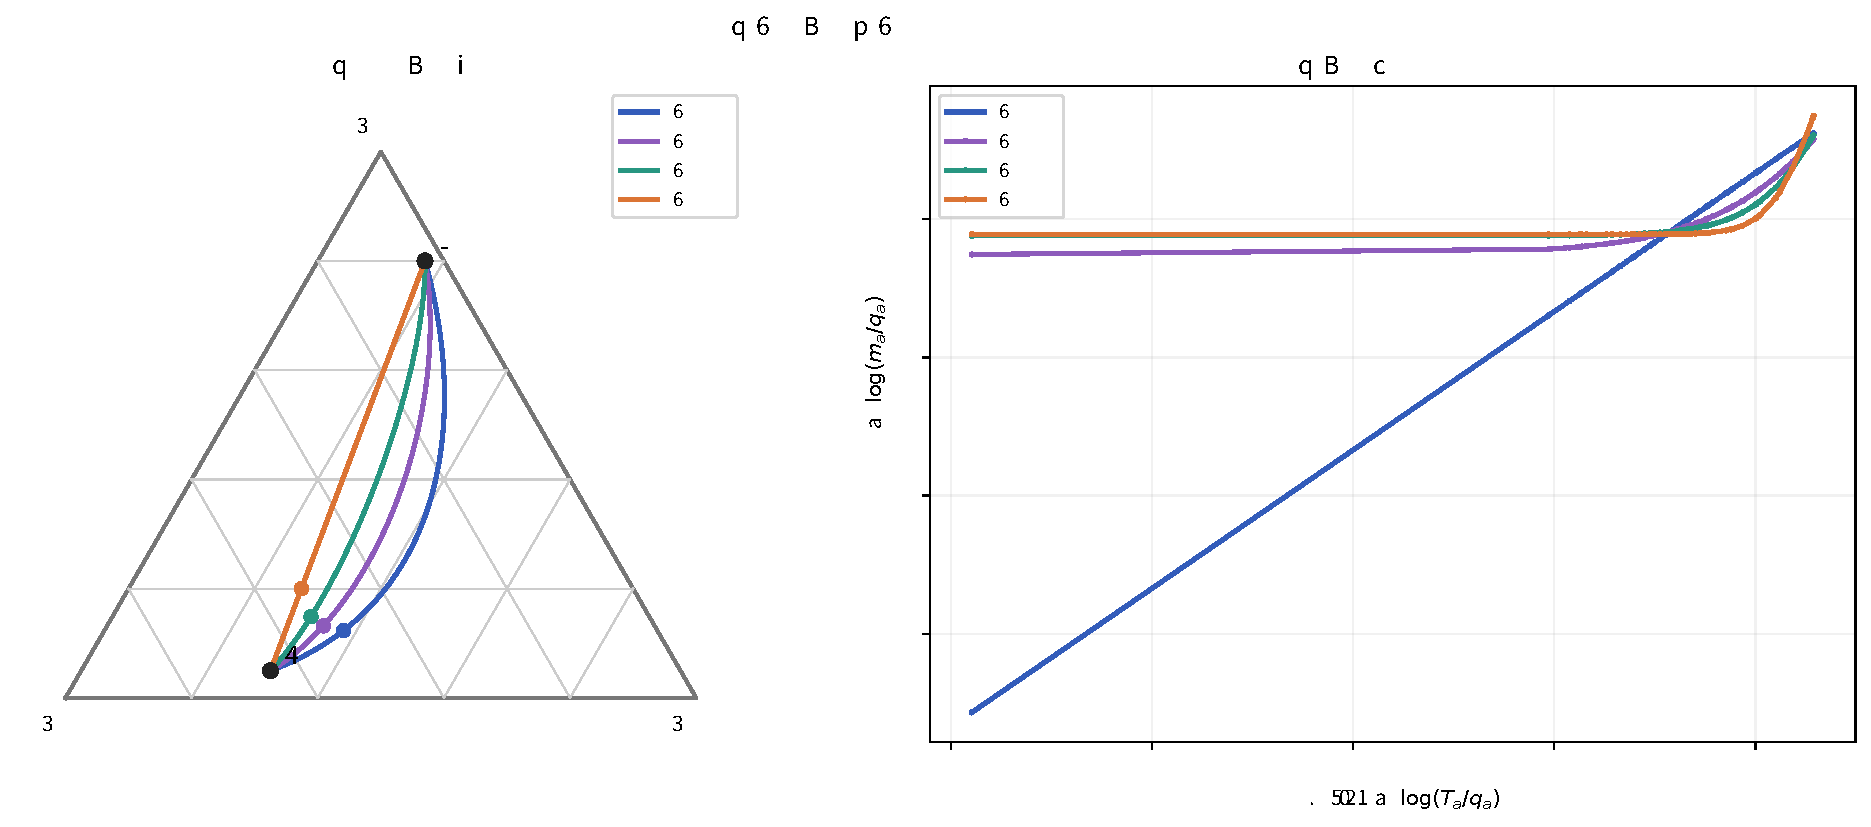
\includegraphics[width=\textwidth]{../../results/proximal-family-geometry/geometry.pdf}
 \caption{幂均值目标 $m_{\kappa,\eta}$ 的概率单纯形路径与 Token 对数概率比。左图圆点均为 $\eta=0.2$；右图展示形状参数 $\kappa>0$ 如何使负尾部平滑饱和，同时在 $\log(t/q)=0$ 附近保持相同的切线斜率。}
\end{figure}

\section{逆向积分定理：幂均值更新是全局教师目标 \texorpdfstring{$\mathcal J_{\kappa,\eta}$}{J(kappa,eta)} 的精确镜像下降}
\label{sec:proximal-md-objective}

定理~\ref{thm:proximal-barycenter-gap} 表明，幂均值目标 $m_{\kappa,\eta}$ 等价于将定理~\ref{thm:ch2-gibbs} 的冻结信号取为 $A_{\kappa,\eta}(t/q)$ 时的标准负熵镜像步：
\begin{equation}
 m_{\kappa,\eta}=\argmax_{p\in\Delta_V}
 \left\{\sum_{a\in\mathcal V} p_a A_{\kappa,\eta}\!\left(\frac{t_a}{q_a}\right)
       -\frac1\eta\KL(p\Vert q)\right\}.
 \label{eq:power-bpo-mirror-subproblem}
\end{equation}
但这里有一个深刻的优化理论问题：因为信号 $A_{\kappa,\eta}(t/q)$ 本身含有 $\eta$ 且是非线性的，当外层反复将锚点同步为 $q_{k+1}=m_{\kappa,\eta}(q_k,t)$ 时，\textbf{整个外层过程究竟是不是某个固定教师目标泛函的标准镜像下降（Mirror Descent）？} 如果是，这个全局教师目标长什么样？

下面的定理通过逆向积分给出了完美的肯定回答：

\begin{theorem}[幂均值信号的可积性、精确 MD 教师目标 $\mathcal J_{\kappa,\eta}$ 与全局收敛率]
\label{thm:power-md-integrable-objective}
\label{thm:power-md-objective-endpoints}
\label{thm:power-md-uniform-cap}
\label{thm:power-md-relative-smoothness}
固定 $\kappa\in[0,1]$ 与 $\eta\in(0,1)$，定义规范化生成函数与全局教师散度目标：
\begin{equation}
 \omega_{\kappa,\eta}(x)
 =x\int_1^x\frac{A_{\kappa,\eta}(u)}{u^2}\,du
 \quad (x>0),
 \qquad
 \mathcal J_{\kappa,\eta}(p;t)
 =D_{\omega_{\kappa,\eta}}(t\Vert p)
 =\sum_{a\in\mathcal V} p_a\omega_{\kappa,\eta}\!\left(\frac{t_a}{p_a}\right).
 \label{eq:power-md-generator-integral}
\end{equation}
该目标泛函具有以下四项核心性质：
\begin{enumerate}
\item \textbf{精确梯度与镜像下降等价性（定理~\ref{thm:power-md-integrable-objective}）}：$\omega_{\kappa,\eta}(1)=\omega_{\kappa,\eta}'(1)=0$，二阶导数满足调和曲率律：
\begin{equation}
 \omega_{\kappa,\eta}''(x)=\frac{A_{\kappa,\eta}'(x)}{x}
 =\frac{x^{\kappa-2}}{1-\eta+\eta x^\kappa}>0
 \qquad\Longleftrightarrow\qquad
 \frac1{\omega_{\kappa,\eta}''(x)}
 =\frac{1-\eta}{g_\kappa''(x)}+\frac\eta{g_0''(x)}.
 \label{eq:power-md-curvature}
\end{equation}
故 $\mathcal J_{\kappa,\eta}(p;t)\ge 0$ 且唯一全局最小点为 $p=t$。在开单纯形上，其概率坐标偏导数恒为
\begin{equation}
 \frac{\partial\mathcal J_{\kappa,\eta}}{\partial p_a}(p;t)
 =-A_{\kappa,\eta}\!\left(\frac{t_a}{p_a}\right).
 \label{eq:power-md-exact-gradient}
\end{equation}
因此，在锚点 $q$ 处对固定目标 $\mathcal J_{\kappa,\eta}(\cdot;t)$ 执行步长为 $\eta$ 的标准负熵镜像步
\begin{equation}
 p^+=\argmin_{p\in\Delta_V}
 \left\{\bigl\langle\nabla_p\mathcal J_{\kappa,\eta}(q;t),\,p-q\bigr\rangle
       +\frac1\eta\KL(p\Vert q)\right\},
 \label{eq:power-md-exact-step}
\end{equation}
其唯一解\textbf{精确等于幂均值目标分布 $m_{\kappa,\eta}(q,t)$}！
\item \textbf{端点闭式解与归一化加权 JS 散度（定理~\ref{thm:power-md-objective-endpoints}）}：当 $\kappa=0$（或 $\eta\to 1$）时，$\mathcal J_{0,\eta}(p;t)=\KL(p\Vert t)$；当 $\eta\to 0^+$ 时，$\lim_{\eta\to 0^+}\mathcal J_{\kappa,\eta}(p;t)=D_\kappa(t\Vert p)$；当 $\kappa=1$ 且固定 $0<\eta<1$ 时，记混合分布 $M=(1-\eta)p+\eta t$，目标闭式解为归一化加权 Jensen--Shannon（JS）散度：
\begin{equation}
 \boxed{\mathcal J_{1,\eta}(p;t)
 =\frac{(1-\eta)\KL(p\Vert M)+\eta\KL(t\Vert M)}{\eta(1-\eta)}.}
 \label{eq:power-md-js-endpoint}
\end{equation}
\item \textbf{分布无关的锐统一上界（定理~\ref{thm:power-md-uniform-cap}）}：当 $0<\kappa\le 1$ 且 $0<\eta<1$ 时，记 $c=c_{\kappa,\eta}=-\frac{\log(1-\eta)}{\kappa\eta}$、$d=\int_1^\infty A_{\kappa,\eta}(u)u^{-2}\,du\le 1/\eta$，则对一切正支持分布恒有 $0\le\mathcal J_{\kappa,\eta}(p;t)\le c+d<\infty$。
\item \textbf{全局 $1/\eta$-相对光滑性与 $O(1/(\eta K_{\mathrm{out}}))$ 外层收敛率（定理~\ref{thm:power-md-relative-smoothness}）}：在开单纯形上，$\mathcal J=\mathcal J_{\kappa,\eta}(\cdot;t)$ 相对于负熵 $H(p)=\sum_a p_a\log p_a$ 满足全局 $1/\eta$-相对光滑性：
\begin{equation}
 \mathcal J(p;t)\le\mathcal J(q;t)+\bigl\langle\nabla\mathcal J(q;t),\,p-q\bigr\rangle
       +\frac1\eta\KL(p\Vert q).
 \label{eq:power-md-relative-smoothness}
\end{equation}
对步长 $0<\tau\le\eta$ 的更新 $p^+\propto q\exp[\tau A_{\kappa,\eta}(t/q)]$，单步下降与三点进展满足：
\begin{align}
 \mathcal J(q;t)-\mathcal J(p^+;t)
 &\ge\frac1\tau\KL(q\Vert p^+)
  +\left(\frac1\tau-\frac1\eta\right)\KL(p^+\Vert q)\ge 0,\\
 \tau\mathcal J(p^+;t)
 &\le\KL(t\Vert q)-\KL(t\Vert p^+).
 \label{eq:power-md-single-step-progress}
\end{align}
特别地，取 $\tau_k\equiv\eta$（即每轮精确更新到幂均值目标 $q_{k+1}=m_{\kappa,\eta}(q_k,t)$），经过 $K_{\mathrm{out}}$ 轮后的末步（Last-Iterate）误差满足：
\begin{equation}
 \mathcal J_{\kappa,\eta}(q_{K_{\mathrm{out}}};t)\le
 \frac{\KL(t\Vert q_0)}{\eta K_{\mathrm{out}}}.
 \label{eq:power-md-last-iterate-rate}
\end{equation}
\end{enumerate}
\end{theorem}
\begin{proof}
（1）对 $\omega(x)=x\int_1^x A(u)u^{-2}\,du$ 求导得 $\omega'(x)=\int_1^x A(u)u^{-2}\,du+A(x)/x$，从而透视函数对 $p_a$ 的偏导数为 $\frac{\partial}{\partial p_a}[p_a\omega(t_a/p_a)]=\omega(x)-x\omega'(x)=-A(x)$（其中 $x=t_a/p_a$）。再求导得 $\omega''(x)=A'(x)/x=x^{\kappa-2}/(1-\eta+\eta x^\kappa)>0$，取倒数即得式~\eqref{eq:power-md-curvature}。将 $\nabla_p\mathcal J(q;t)=-A(t/q)$ 代入镜像步~\eqref{eq:power-md-exact-step}，由定理~\ref{thm:ch2-gibbs} 立得 $p^+=m_{\kappa,\eta}$。
（2）对 $\kappa=1$ 分部积分计算 $\omega_{1,\eta}(x)=\frac{\eta x\log x-(1-\eta+\eta x)\log(1-\eta+\eta x)}{\eta(1-\eta)}$，代入求和即得加权 JS 散度~\eqref{eq:power-md-js-endpoint}。
（3）由凸函数渐近斜率性质 $\omega(x)\le\lim_{u\to 0^+}\omega(u)+x\lim_{u\to\infty}\frac{\omega(u)}{u}=c+dx$ 对 $x=t/p$ 求 $p$-期望即得统一上界 $c+d$。
（4）记 $x_a=t_a/p_a$，由式~\eqref{eq:power-md-curvature} 可得单纯形上的对角 Hessian 上界：
\begin{equation}
 \nabla_p^2\mathcal J(p;t)
 =\operatorname{diag}\left(\frac1{p_a}
       \frac{x_a^\kappa}{1-\eta+\eta x_a^\kappa}\right)
 \preceq\frac1\eta\operatorname{diag}\left(\frac1{p_a}\right)
 =\frac1\eta\nabla^2 H(p).
 \label{eq:power-md-hessian-bound}
\end{equation}
积分二阶泰勒余项即得式~\eqref{eq:power-md-relative-smoothness}。结合 MD 一阶条件 $\langle\nabla\mathcal J(q;t),p^+-q\rangle=-\tau^{-1}[\KL(p^+\Vert q)+\KL(q\Vert p^+)]$、目标凸性 $\mathcal J(q;t)\le\langle\nabla\mathcal J(q;t),q-t\rangle$ 及 Bregman 三点恒等式，立得式~\eqref{eq:power-md-single-step-progress}。对 $k=0,\ldots,K_{\mathrm{out}}-1$ 望远镜求和并利用 $\mathcal J(q_k;t)$ 的单调非增性即得式~\eqref{eq:power-md-last-iterate-rate}。
\end{proof}


\chapter{为什么“不一步到教师”且取 \texorpdfstring{$\kappa\le 1/2$}{kappa <= 1/2} 更稳定？（方差相变与平方根最优性）}
\label{ch:variance-stability}

前一章从优化角度证明了 $(\kappa,\eta)$ 目标对应全局教师散度 $\mathcal J_{\kappa,\eta}$ 的精确镜像下降。本章从\textbf{统计方差与动态收敛稳定性}角度回答核心问题：为什么在 $0<\eta<1$ 下必须选择 $0<\kappa\le 1/2$？为什么平方根形状 $\kappa=1/2$ 是兼具方差有界性、误差自界性与全局几何收缩的黄金工作点？

\section{二阶矩形状相变定理：为什么 \texorpdfstring{$\kappa=1/2$}{kappa=1/2} 是小步方差有界的精确分界线？}
\label{sec:proximal-teacher-center}

首先，对于任意固定的正插值强度 $0<\eta<1$ 和任意正形状 $0<\kappa\le 1$，未归一化信号 $f_{\kappa,\eta}(r)=\kappa^{-1}\log(1-\eta+\eta e^{\kappa r})$ 与归一化监督 $A_{\kappa,\eta}=f_{\kappa,\eta}/\eta$ 均具有不依赖词表维数的有限二阶矩上界：

\begin{theorem}[固定正步长 $\eta\in(0,1)$ 下幂均值信号的统一二阶矩上界]
\label{thm:proximal-power-variance}
设有限词表上 $q_a,t_a>0$，$0<\kappa\le 1$，$0<\eta<1$。定义有限通用常数：
\begin{equation}
 C_\star=\sup_{u>0}\frac{\log^2(1+u)}{u}<\infty,\qquad
 B_{\kappa,\eta}=\frac{\log^2(1-\eta)+C_\star\eta}{\kappa^2}.
\end{equation}
则对任意分布 $(q,t)$，恒有 $\E_q[f_{\kappa,\eta}^2]\le B_{\kappa,\eta}$ 与 $\E_q[A_{\kappa,\eta}^2]\le B_{\kappa,\eta}/\eta^2$。若得分向量满足 $\|\psi(a)\|\le S$，则中心化教师得分梯度的协方差迹满足 $\Var_q[\psi C_q A_{\kappa,\eta}]\le S^2\Var_q(A_{\kappa,\eta})\le S^2 B_{\kappa,\eta}/\eta^2$。
\end{theorem}
\begin{proof}
记 $\rho=t/q$。在负区域 $\rho<1$ 上，因 $\log(1-\eta)/\kappa\le f_{\kappa,\eta}<0$，平方期望不超过 $\log^2(1-\eta)/\kappa^2$；在正区域 $\rho\ge 1$ 上，$0\le f_{\kappa,\eta}\le\kappa^{-1}\log(1+\eta\rho^\kappa)$，故 $f_{\kappa,\eta}^2\le C_\star\eta\rho^\kappa/\kappa^2$。由 $0<\kappa\le 1$ 时 $x^\kappa$ 的凹性与 $\E_q[\rho]=1$，Jensen 不等式给出 $\E_q[\rho^\kappa]\le 1$，合并两区域即得结论。
\end{proof}

然而，定理~\ref{thm:proximal-power-variance} 中 $A_{\kappa,\eta}$ 的上界 $B_{\kappa,\eta}/\eta^2$ 在小步长 $\eta\to 0$ 时粗看似乎按 $\Theta(\eta^{-1})$ 发散。那么，当我们在精细步长（小 $\eta$）下运行多步蒸馏时，哪些形状参数 $\kappa$ 才能真正保证归一化监督 $A_{\kappa,\eta}$ 的最坏方差不随 $\eta\to 0$ 爆炸？下面的相变定理给出了精确的充要条件：

\begin{theorem}[小步极限下最坏二阶矩与 $p$ 阶矩的精确形状相变阈值]
\label{thm:proximal-moment-threshold}
\label{thm:power-general-moment-threshold}
定义完整支持分布类上的最坏未归一化信号二阶矩 $\mathcal B_\kappa(\eta)=\sup_{q,t\in\Delta_V^\circ}\E_q[f_{\kappa,\eta}^2]$。对任意固定形状 $0<\kappa\le 1$，当 $\eta\to 0^+$ 时，成立精确渐近阶数：
\begin{align}
 \mathcal B_\kappa(\eta)&=\Theta_\kappa\!\left(\eta^{\min\{2,\,1/\kappa\}}\right),
 \label{eq:proximal-sharp-moment-order}\\
 \sup_{q,t}\E_q\bigl|A_{\kappa,\eta}\bigr|^p
 &=\Theta_{\kappa,p}\!\left(\eta^{\min\{p,\,1/\kappa\}-p}\right),
 \qquad
 \sup_{q,t}\Var_q(A_{\kappa,\eta})
 =\Theta_\kappa\!\left(\eta^{\min\{2,\,1/\kappa\}-2}\right)\quad(p\ge 1).
\end{align}
因此，幂均值族在小步极限下呈现鲜明的\textbf{方差相变（Phase Transition）}：
\begin{enumerate}
\item 当且仅当 \textbf{$0<\kappa\le 1/2$} 时，$\mathcal B_\kappa(\eta)=\Theta_\kappa(\eta^2)$，归一化监督 $A_{\kappa,\eta}$ 与中心化监督 $C_q A_{\kappa,\eta}$ 的最坏二阶矩在 $\eta\to 0^+$ 时保持为 \textbf{$O_\kappa(1)$ 有限常数}！（一般 $p$ 阶矩保持 $O(1)$ 的充要区间为 $0<\kappa\le 1/p$。）
\item 当 \textbf{$1/2<\kappa\le 1$}（含算术混合 $\kappa=1$）时，稀有锚点动作（$q_a\to 0$）的正尾部主导二阶矩，导致 $\sup_{q,t}\Var_q(A_{\kappa,\eta})=\Theta_\kappa(\eta^{1/\kappa-2})\to\infty$（例如算术端点 $\kappa=1$ 按 $\Theta(\eta^{-1})$ 发散）。
\item 当 \textbf{$\kappa=0$}（标准几何 OPD）时，负尾部无界导致对任意 $\eta>0$ 均有 $\mathcal B_0(\eta)=\infty$。
\end{enumerate}
\end{theorem}
\begin{proof}
负区域 $\rho<1$ 对 $\E_q|f|^p$ 的贡献恒不超过 $|\log(1-\eta)/\kappa|^p=O_{\kappa,p}(\eta^p)$。
\begin{itemize}
\item 当 $p\kappa\le 1$（二阶矩 $p=2$ 时即 $0<\kappa\le 1/2$）：在正区域 $\rho\ge 1$ 上使用 $\log(1+x)\le x$ 及凹函数 Jensen 不等式 $\E_q[\rho^{p\kappa}]\le(\E_q[\rho])^{p\kappa}=1$，立得 $\E_q[|f|^p\mathbf1\{\rho\ge 1\}]\le\frac{\eta^p}{\kappa^p}\E_q[\rho^{p\kappa}]\le\frac{\eta^p}{\kappa^p}$。同除以 $\eta^p$ 即证 $\sup_{q,t}\E_q|A_{\kappa,\eta}|^p=O_{\kappa,p}(1)$。
\item 当 $p\kappa>1$（二阶矩 $p=2$ 时即 $1/2<\kappa\le 1$）：令 $s=1/\kappa\in[1,p)$，则 $C_{p,s}=\sup_{x>0}\frac{\log^p(1+x)}{x^s}<\infty$。正区域期望不超过 $\frac{C_{p,s}\eta^s}{\kappa^p}\E_q[\rho^{\kappa s}]=\frac{C_{p,s}}{\kappa^p}\eta^{1/\kappa}$。为证下界达到该阶数，构造随 $\eta$ 变化的二元分布 $t=(1/2,1/2),\; q_1=\frac12\eta^{1/\kappa},\; q_2=1-q_1$。此时稀有动作满足 $\rho_1=\eta^{-1/\kappa}$、$f_1=\frac{\log(2-\eta)}{\kappa}$，故 $\E_q|f|^p\ge q_1|f_1|^p=\frac{\eta^{1/\kappa}}{2\kappa^p}\log^p(2-\eta)=\Omega_{\kappa,p}(\eta^{1/\kappa})$。同除以 $\eta^p$ 即得 $\Theta_{\kappa,p}(\eta^{1/\kappa-p})$。
\end{itemize}
\end{proof}

\begin{figure}[htbp]
 \centering
 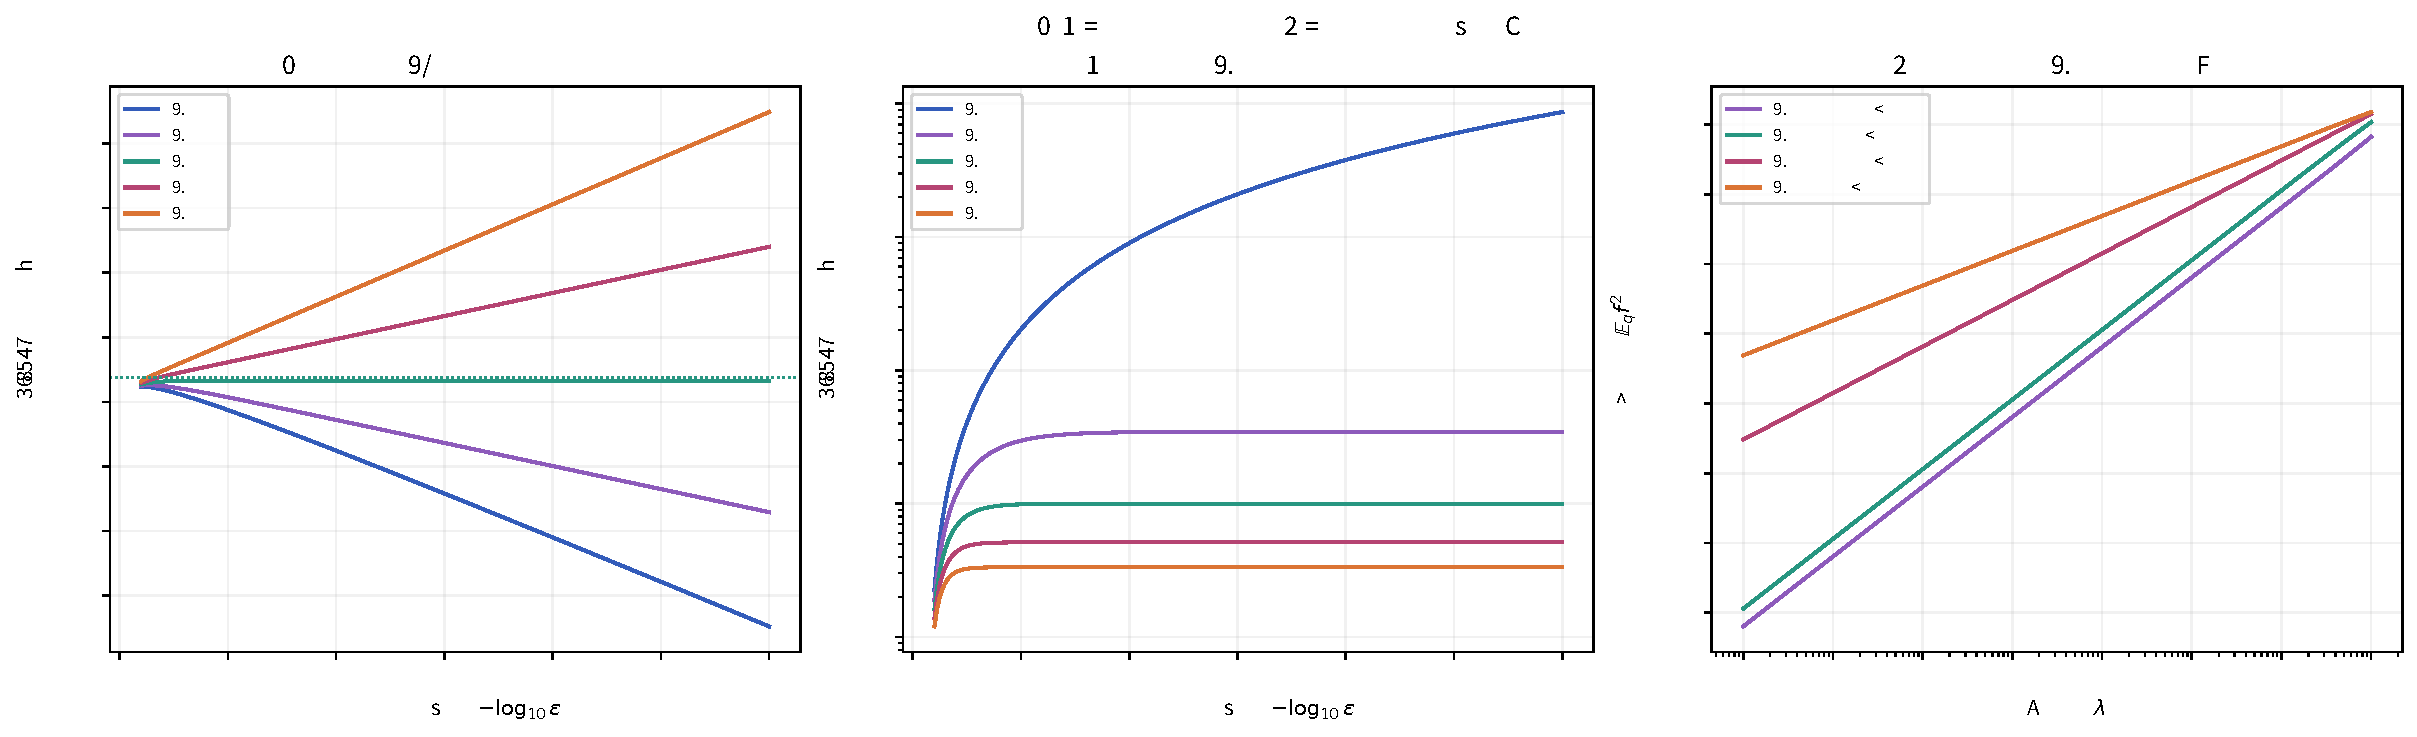
\includegraphics[width=\textwidth]{../../results/proximal-family-geometry/threshold.pdf}
 \caption{形状相变阈值 $\kappa=1/2$ 的解析验证。左图：当学生动作概率趋零时，$\kappa>1/2$ 的自然梯度速度发散；中图：当教师动作概率趋零时，几何端点 $\kappa=0$ 的速度发散；右图：二阶矩对数斜率在 $\kappa=0.25,0.5,0.75,1.0$ 处精确等于 $\min\{2,1/\kappa\}=\{2,2,4/3,1\}$。}
\end{figure}

\section{误差自界（Error-Scaled）方差控制：越接近教师，监督噪声越小}

在 $0<\kappa\le 1/2$ 的稳定区间内，幂均值监督不仅具有分布无关的常数方差上界，而且与冻结教师中心
\begin{equation}
 \boxed{K_{\kappa,\eta}(q,t)
 =-\E_q\bigl[A_{\kappa,\eta}(\rho)\bigr]
 =\E_q\bigl[\phi_{\kappa,\eta}(t/q)\bigr],\qquad
 \phi_{\kappa,\eta}(x)=x-1-\frac{\log(1-\eta+\eta x^\kappa)}{\kappa\eta}}
 \label{eq:center-expanded-k}
\end{equation}
之间存在深刻的\textbf{自界（Self-Bounding）耦合关系}。

\begin{theorem}[教师中心的有界性、误差相关方差自界与全训练周期可求和噪声]
\label{thm:center-bounds-monotonicity}
\label{thm:center-advantage-variance}
\label{thm:power-md-center-comparison}
\label{cor:power-md-summable-variance}
设 $0<\kappa\le 1/2$ 且 $0<\eta<1$，记 $a_\kappa=\sum_a q_a^{1-\kappa}t_a^\kappa$，中心化教师优势方差为 $V_{\kappa,\eta}=\Var_q(B_{\kappa,\eta})=\Var_q(A_{\kappa,\eta})$。则：
\begin{enumerate}
\item \textbf{教师中心的凸散度界与 MD 目标等价性（定理~\ref{thm:center-bounds-monotonicity}、\ref{thm:power-md-center-comparison}）}：$\phi_{\kappa,\eta}(1)=\phi_{\kappa,\eta}'(1)=0$ 且 $\phi_{\kappa,\eta}''(x)>0$，故 $K_{\kappa,\eta}(q,t)\ge 0$（当且仅当 $q=t$ 时为零），关于 $\kappa$ 单调非增、关于 $\eta$ 单调非减，且同时满足分布无关上界与 MD 目标夹逼不等式：
\begin{equation}
 (1-\kappa)D_\kappa(t\Vert q)\le K_{\kappa,\eta}(q,t)\le\min\bigl\{\KL(q\Vert t),\; c_{\kappa,\eta}\bigr\},
 \qquad
 (1-\kappa)\mathcal J_{\kappa,\eta}(q;t)\le K_{\kappa,\eta}(q,t)\le\mathcal J_{\kappa,\eta}(q;t).
 \label{eq:center-uniform-cap}
\end{equation}
\item \textbf{监督方差受当前教师误差线性控制（定理~\ref{thm:center-advantage-variance}）}：$V_{\kappa,\eta}$ 同时满足统一常数界与误差自界：
\begin{equation}
 V_{\kappa,\eta}
 \le\frac{1-a_\kappa^2}{\kappa^2(1-\eta)^2}
 \le\frac1{\kappa^2(1-\eta)^2},
 \qquad
 \boxed{V_{\kappa,\eta}
 \le\frac{D_\kappa(t\Vert q)}{\kappa(1-\eta)^2}
 \le\frac{K_{\kappa,\eta}(q,t)}{\kappa(1-\kappa)(1-\eta)^2}.}
 \label{eq:center-error-scaled-variance}
\end{equation}
\item \textbf{精确外层迭代下的监督方差按 $O(1/K_{\mathrm{out}})$ 衰减且全周期可求和（推论~\ref{cor:power-md-summable-variance}）}：在精确幂均值外层更新 $q_{k+1}=m_{\kappa,\eta}(q_k,t)$ 下，记 $C_0=\KL(t\Vert q_0)$，第 $k$ 轮方差 $V_k$ 满足：
\begin{equation}
 V_{K_{\mathrm{out}}}\le\frac{C_0}{\kappa(1-\kappa)(1-\eta)^2\eta K_{\mathrm{out}}},
 \qquad
 \sum_{k=1}^{K_{\mathrm{out}}} V_k\le\frac{C_0}{\kappa(1-\kappa)(1-\eta)^2\eta}<\infty.
 \label{eq:power-md-summable-variance}
\end{equation}
\end{enumerate}
\end{theorem}
\begin{proof}
（1）由 $\phi_{\kappa,\eta}''(x)=\frac{x^{\kappa-2}[(1-\kappa)(1-\eta)+\eta x^\kappa]}{(1-\eta+\eta x^\kappa)^2}$ 与 $\omega_{\kappa,\eta}''(x)$ 的比值属于 $[1-\kappa,1]$，积分两次即得夹逼式~\eqref{eq:center-uniform-cap}。
（2）令 $X=\rho^\kappa\ge 0$，$h(X)=\frac{\log(1-\eta+\eta X)}{\kappa\eta}$。因 $|h'(X)|\le\frac{1}{\kappa(1-\eta)}$，有 $V_{\kappa,\eta}=\Var_q(h(X))\le\frac{\Var_q(X)}{\kappa^2(1-\eta)^2}$。考察凸矩函数 $a(u)=\E_q[\rho^u]$（$a''(u)\ge 0, a(1)=1$），因 $2\kappa\in[\kappa,1]$，弦线不等式给出 $a(2\kappa)\le\frac{1-2\kappa}{1-\kappa}a(\kappa)+\frac{\kappa}{1-\kappa}$，故
\begin{equation*}
 \Var_q(X)=a(2\kappa)-a(\kappa)^2
 \le\frac{\bigl[1-a(\kappa)\bigr]\bigl[\kappa+(1-\kappa)a(\kappa)\bigr]}{1-\kappa}
 \le\frac{1-a(\kappa)}{1-\kappa}=\kappa D_\kappa(t\Vert q).
\end{equation*}
除以 $\kappa^2(1-\eta)^2$ 并结合 $(1-\kappa)D_\kappa\le K_{\kappa,\eta}$ 即得自界式~\eqref{eq:center-error-scaled-variance}。
（3）将 $V_k\le\frac{K_k}{\kappa(1-\kappa)(1-\eta)^2}\le\frac{\mathcal J(q_k;t)}{\kappa(1-\kappa)(1-\eta)^2}$ 代入定理~\ref{thm:power-md-relative-smoothness} 的三点望远镜和 $\eta\sum_{k=1}^{K_{\mathrm{out}}}\mathcal J(q_k;t)\le C_0$ 即得式~\eqref{eq:power-md-summable-variance}。
\end{proof}

\begin{figure}[htbp]
 \centering
 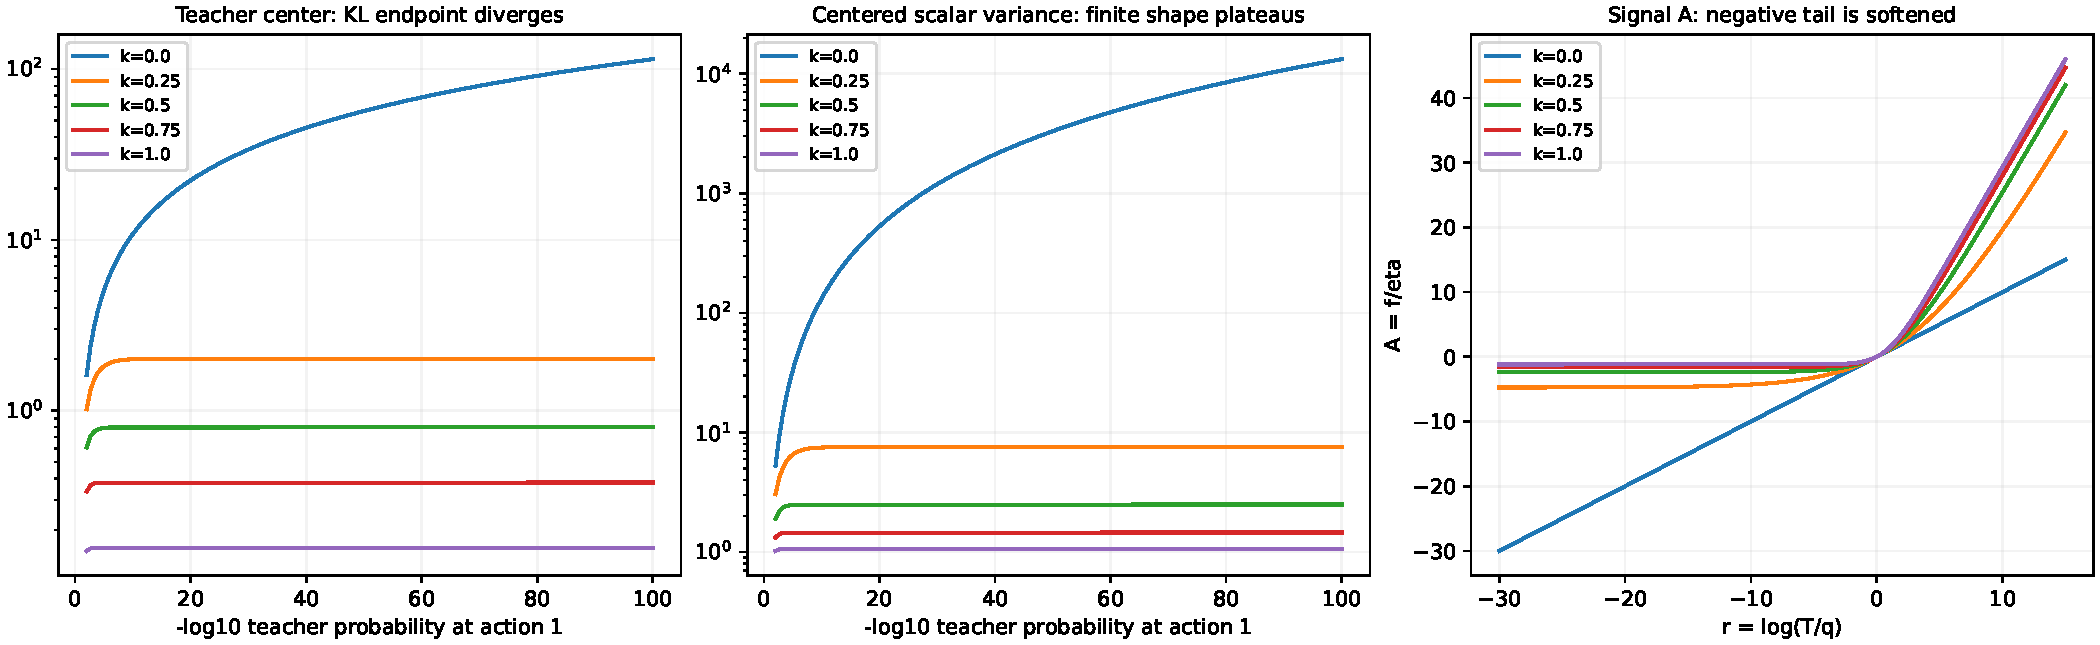
\includegraphics[width=\textwidth]{../../results/power-center-advantage/negative-tail-center-variance.pdf}
 \caption{固定 $q=(1/2,1/2),\;\eta=0.3$，当教师一个动作概率趋零时，标准几何中心（$\kappa=0$）及优势方差发散至无穷大，而正形状（$\kappa>0$）稳定在有界平台。}
\end{figure}

\section{平方根形状（\texorpdfstring{$\kappa=1/2$}{kappa=1/2}）的相对噪声最优性与显式 Hellinger 收缩}
\label{sec:power-half-and-optimality}

在有界方差区间 $0<\kappa\le 1/2$ 内部，我们应该选择哪个具体的 $\kappa$？本节证明：\textbf{平方根形状 $\kappa=1/2$} 不仅位于相变边界的最大允许值处，而且同时具备两项独一无二的理论优势。

\begin{theorem}[平方根形状 $\kappa=1/2$ 的相对误差噪声最优性与全局 $(1-\eta)$ Hellinger 收缩]
\label{thm:power-relative-noise-optimum}
\label{thm:power-half-discrete-contraction}
\label{cor:power-half-geometric-noise}
\label{thm:power-common-local-rate}
\begin{enumerate}
\item \textbf{相对教师误差的最坏噪声放大常数唯一最优（定理~\ref{thm:power-relative-noise-optimum}）}：对 $0<\kappa\le 1/2$，令小步监督为 $A_\kappa^0=(\rho^\kappa-1)/\kappa$，小步中心为 $K_\kappa^0=(1-\E_q[\rho^\kappa])/\kappa$。在全体严格正且 $q\ne t$ 的分布对上取上确界，有精确锐常数：
\begin{equation}
 \sup_{q\ne t}\frac{\Var_q(A_\kappa^0)}{D_\kappa(t\Vert q)}=\frac1\kappa,\qquad
 \sup_{q\ne t}\frac{\Var_q(A_\kappa^0)}{K_\kappa^0}=\frac1{\kappa(1-\kappa)}.
 \label{eq:power-relative-noise-sharp}
\end{equation}
在整个 $\kappa\in[0,1]$ 族中，上述两个相对噪声准则均由 \textbf{$\kappa=1/2$ 唯一最小化}（最小锐常数分别为 $2$ 和 $4$；而在 $\kappa=0$ 或 $\kappa>1/2$ 处上确界均为 $+\infty$）。（注：若改为不除以教师散度、单纯最小化绝对小步方差上确界 $\sup_{q,t}\Var_q(A_\kappa^0)=C_{\mathrm{vel}}(\kappa)=\frac{b^{1-2\kappa}(1-b)}{\kappa^2},\; b=\frac{1-2\kappa}{2(1-\kappa)}$，则唯一极小极大点位于 $\kappa_\star\approx 0.4419283735$，对应值 $3.527275$，与 $\kappa=1/2$ 处的 $4$ 十分接近。）
\item \textbf{显式 $(1-\eta)$ 全局 Hellinger 几何收缩与无初始 KL 依赖的方差和（定理~\ref{thm:power-half-discrete-contraction}、推论~\ref{cor:power-half-geometric-noise}）}：记亲和度 $a=\sum_v\sqrt{q_v t_v}$、平方 Hellinger 距离 $H^2(q,t)=\sum_v(\sqrt{q_v}-\sqrt{t_v})^2=2(1-a)\le 2$。单步精确平方根目标 $m=m_{1/2,\eta}(q,t)$ 在正单位球面上满足：
\begin{equation}
 \sqrt{m_{1/2,\eta}}=\frac{(1-\eta)\sqrt{q}+\eta\sqrt{t}}{\sqrt{Z}},
 \qquad a^+=\sum_v\sqrt{m_v t_v}=\frac{(1-\eta)a+\eta}{\sqrt{Z}}\ge(1-\eta)a+\eta,
 \label{eq:power-half-normalized-chord}
\end{equation}
从而成立无需任何最小概率下界假设的\textbf{全局几何收缩与有界累计方差}：
\begin{equation}
 \boxed{\begin{aligned}
 H^2(m,t)&\le(1-\eta)H^2(q,t),\\
 H^2(q_k,t)&\le(1-\eta)^k H^2(q_0,t),\\
 \sum_{k=0}^\infty V_k&\le\frac{4H^2(q_0,t)}{\eta(1-\eta)^2}\le\frac{8}{\eta(1-\eta)^2}.
 \end{aligned}}
 \label{eq:power-half-discrete-progress}
\end{equation}
（其连续自然梯度流则满足精确解析解 $a(\tau_{\mathrm{flow}})=\tanh(\tau_{\mathrm{flow}}+\operatorname{artanh}a(0))$。）
\item \textbf{教师邻域的局部收敛率不变性（定理~\ref{thm:power-common-local-rate}）}：当 $q=t+\epsilon h$（$\sum_a h_a=0,\;\epsilon\to 0$）接近教师时，所有形状 $\kappa\in[0,1]$ 的幂均值目标共享完全相同的一阶线性项 $m_a=t_a+(1-\eta)\epsilon h_a+O(\epsilon^2)$，因此在任意光滑评价散度 $D_g$ 下的局部渐近单步收缩率恒为 $\lim_{\epsilon\to 0}\frac{D_g(m\Vert t)}{D_g(q\Vert t)}=(1-\eta)^2$。
\end{enumerate}
\end{theorem}
\begin{proof}
（1）上界已由定理~\ref{thm:center-advantage-variance} 给出；下界锐性由二元分布族 $q=(v,1-v),\; t=(v^2,1-v^2)$ 在 $v\downarrow 0$ 时的泰勒展开 $\Var_q(A_\kappa^0)=v/\kappa^2+o(v),\; D_\kappa=v/\kappa+o(v),\; K_\kappa^0=(1-\kappa)v/\kappa+o(v)$ 精确达到。
（2）将式~\eqref{eq:power-half-normalized-chord} 与 $\sqrt{t}$ 做内积得 $a^+=[(1-\eta)a+\eta]/\sqrt{Z}$。因 $a\le 1\implies Z=(1-\eta)^2+\eta^2+2\eta(1-\eta)a\le[(1-\eta)+\eta]^2=1$，故 $a^+\ge(1-\eta)a+\eta\implies 1-a^+\le(1-\eta)(1-a)$，两边乘以 $2$ 即得 $H^2(m,t)\le(1-\eta)H^2(q,t)$。代入 $V_k\le\frac{4H^2(q_k,t)}{(1-\eta)^2}$ 并对几何级数 $\sum_{k=0}^\infty(1-\eta)^k=1/\eta$ 求和即得式~\eqref{eq:power-half-discrete-progress}。
（3）对 $[(1-\eta)(t_a+\epsilon h_a)^\kappa+\eta t_a^\kappa]^{1/\kappa}$ 做二阶展开得 $m_a=t_a+(1-\eta)\epsilon h_a+\frac{(\kappa-1)(1-\eta)\eta}{2}\epsilon^2(\frac{h_a^2}{t_a}-t_a\sum_b\frac{h_b^2}{t_b})+O(\epsilon^3)$，一阶项与 $\kappa$ 无关，故二阶散度比值恒为 $(1-\eta)^2$。
\end{proof}

\begin{figure}[H]
 \centering
 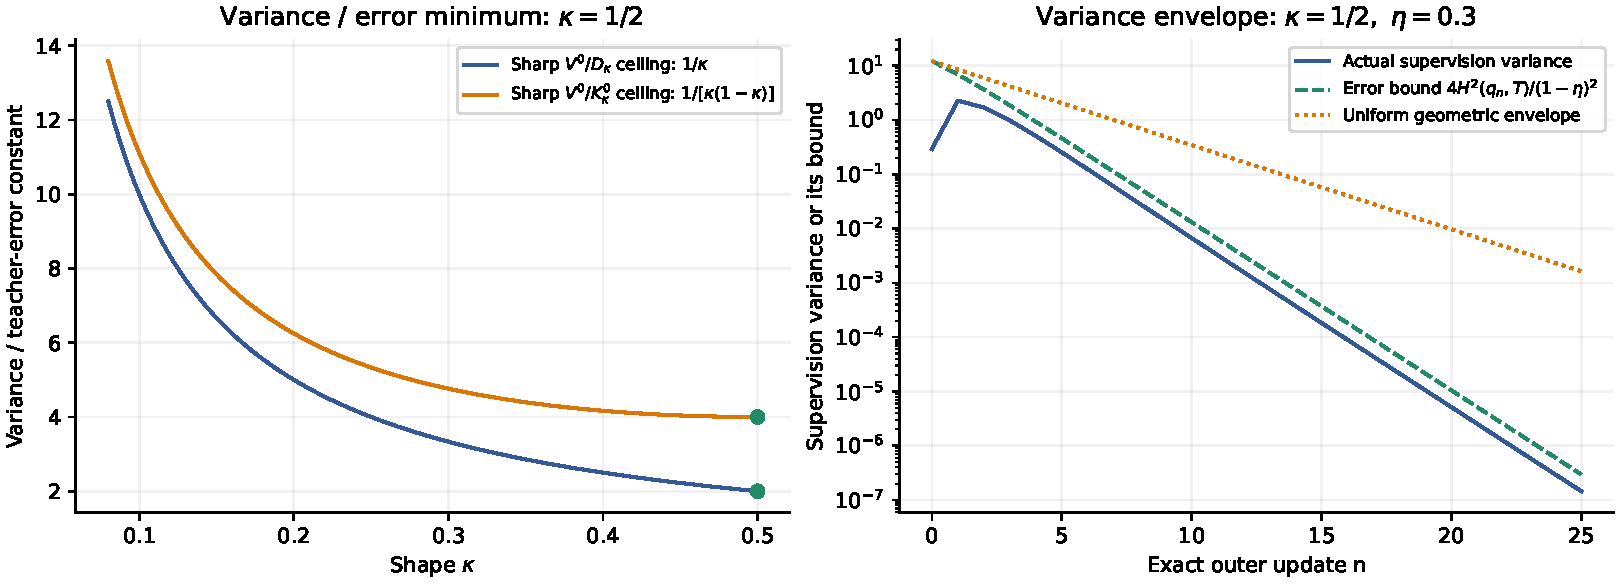
\includegraphics[width=\textwidth]{../../results/chapter9-restructure/relative-noise-and-convergence.pdf}
 \caption{左图：相对教师散度误差的锐噪声常数 $1/\kappa$ 与 $1/[\kappa(1-\kappa)]$ 均在平方根点 $\kappa=1/2$ 处取得唯一最小值。右图：精确平方根外层迭代下，Hellinger 驱动的方差上界按 $(1-\eta)^k$ 严格几何衰减。}
 \label{fig:power-relative-noise-convergence}
\end{figure}

% ============================================================================
% CHAPTER 4: 固定 Rollout 下的四种内层投影目标：商空间统一分解与对比
% ============================================================================
\chapter{固定 Rollout 下的四种内层投影目标：商空间统一分解与对比}
\label{ch:inner-targets}

在前三章中，我们确定了外层第 $k$ 轮锚点 $q=q_k$ 与教师 $t$ 诱导的目标分布（标准对数几何插值目标 $p^{\mathrm G}\propto q\exp(G)$ 或广义 $(\kappa,\eta)$-幂均值目标 $m_{\kappa,\eta}$）。然而，在神经网络参数化的学生策略 $p_\theta$ 上，要在\textbf{同一个固定 rollout 批次}上执行 $N>1$ 步内层更新，我们必须回答第二个核心问题：
\begin{quote}
\textbf{核心问题 2（内层投影与归一化坐标选择）：}在每个固定 prefix 上，目标分布与当前学生分布 $p$ 之间仅在“消去常数偏移的商空间”中唯一对应。不同的归一化方式（配分函数对数、锚点期望中心化、成对差分或学生自身中心化）会诱导出哪几种内层优化目标？为什么在复用冻结 rollout $q$ 时，基于锚点测度 $q$ 的回归投影（BPO / PMD-Mean）比依赖学生分布 $p$ 的重加权更新（MDPO / Token-IS）显著更稳定？
\end{quote}

本章首先建立全耦合商空间坐标双射，将 \textbf{PMD-Part}、\textbf{PMD-Mean}、\textbf{BPO} 与 \textbf{MDPO} 四种内层损失统一表示为同一个中心化残差向量 $E=C_q(U-G)$ 上的不同几何惩罚函数；随后给出各自的精确梯度、停止梯度（stop-gradient）实现与伪代码，并深入剖析 PMD-Mean 的 Lambert-$W$ 精确解、混合 $\KL$--$\chi^2$ 变分刻画及大步长极限。

\section{商空间坐标双射与四种内层损失的统一分解}
\label{sec:quotient-bijection}

固定单个 prefix，记锚点分布 $q\in\Delta^\circ(\mathcal V)$，冻结优势信号为 $f:a\mapsto f(a)$，中心化目标信号为
\begin{equation}
 G(a)=\eta\,C_q f(a)=\eta\bigl(f(a)-\E_q[f]\bigr),
 \qquad \E_q[G]=0.
\end{equation}
对于标准对数几何步（$\kappa=0$），$f(a)=\log(t(a)/q(a))$；对于广义 $(\kappa,\eta)$-幂均值步（$\kappa\in(0,1)$），由\cref{sec:power-bpo-inner} 可知只需将 $G$ 替换为刷新优势 $G_{\kappa,\eta}(a)=\frac{1}{\kappa}C_q\log\bigl((1-\eta)+\eta(t(a)/q(a))^\kappa\bigr)$，其对应的 Gibbs 目标即恰为幂均值重心 $m_{\kappa,\eta}$。因此，本章以统一的零均值冻结目标信号 $G$（满足 $\E_q[G]=0$）展开全部内层理论，所有结论直接同时涵盖 $\kappa=0$ 与 $\kappa\in(0,1)$。

记对应的目标 Gibbs 分布与配分函数对数修正量为
\begin{equation}
 p^{\mathrm G}(a)=\frac{q(a)e^{G(a)}}{Z_q(G)},
 \qquad
 Z_q(G)=\E_q[e^G],
 \qquad
 \Delta=\log Z_q(G)=\KL(q\Vert p^{\mathrm G})\ge 0.
 \label{eq:ch4-gibbs-delta}
\end{equation}
记学生相对锚点的对数比（log-ratio）为 $U(a)=\log\bigl(p(a)/q(a)\bigr)$，其锚点中心化坐标与未中心化残差分别为
\begin{equation}
 X=C_q U=U-\E_q[U],
 \qquad
 D=U-G,
 \qquad
 E=C_q D=X-G.
 \label{eq:ch4-coordinates}
\end{equation}
由于 $p\in\Delta^\circ(\mathcal V)$ 满足归一化约束 $\E_q[e^U]=1$，坐标 $U$ 并非自由向量，而是完全由其零均值商空间坐标 $X\in\mathcal H_0=\{x\in\R^{\mathcal V}:\E_q[x]=0\}$ 唯一决定：

\begin{theorem}[全耦合商空间坐标双射]
\label{thm:quotient-bijection}
对任意 $q\in\Delta^\circ(\mathcal V)$，映射 $p\mapsto X=C_q\log(p/q)$ 是从开单纯形 $\Delta^\circ(\mathcal V)$ 到零均值超平面 $\mathcal H_0$ 的光滑双射，其逆映射与对数比还原公式为
\begin{equation}
 p(a)=\frac{q(a)e^{X(a)}}{\E_q[e^X]},
 \qquad
 U(a)=X(a)-\log\E_q[e^X],
 \qquad
 \KL(q\Vert p)=-\E_q[U]=\log\E_q[e^X].
 \label{eq:quotient-inverse}
\end{equation}
进一步，在中心化残差 $E=X-G\in\mathcal H_0$ 下，未中心化残差 $D=U-G$ 与学生对目标的反向/前向 KL 散度具有如下精确表示：
\begin{align}
 D(a) &= E(a)-\log\E_q[e^{G+E}], \label{eq:quotient-D-from-E}\\
 \KL(q\Vert p) &= \Delta+\log\E_{p^{\mathrm G}}[e^E], \label{eq:quotient-kl-qp}\\
 \KL(p^{\mathrm G}\Vert p) &= \log\E_{p^{\mathrm G}}[e^E]-\E_{p^{\mathrm G}}[E], \label{eq:quotient-kl-pgp}\\
 \KL(p\Vert p^{\mathrm G}) &= \frac{\E_{p^{\mathrm G}}[E e^E]}{\E_{p^{\mathrm G}}[e^E]}-\log\E_{p^{\mathrm G}}[e^E]. \label{eq:quotient-kl-ppg}
\end{align}
特别地，$p=p^{\mathrm G}$ 当且仅当 $X=G$（即 $E=0$），也当且仅当 $D\equiv -\Delta$ 为常数向量。
\end{theorem}
\begin{proof}
若 $C_q\log(p_1/q)=C_q\log(p_2/q)$，则 $\log p_1-\log p_2=c\mathbf 1$，由 $\sum_a p_1(a)=\sum_a p_2(a)=1$ 知 $c=0$，故单射成立；任取 $X\in\mathcal H_0$，定义 $p\propto q e^X$ 即满足 $C_q\log(p/q)=X$，故满射成立。对 $p=q e^U$ 取 $q$-期望得 $1=\E_q[e^U]=e^{\E_q[U]}\E_q[e^X]$，故 $\E_q[U]=-\log\E_q[e^X]$，从而 $U=X-\log\E_q[e^X]$ 且 $\KL(q\Vert p)=-\E_q[U]=\log\E_q[e^X]$。将 $X=G+E$ 代入 $\E_q[e^X]=Z_q(G)\E_{p^{\mathrm G}}[e^E]=e^\Delta\E_{p^{\mathrm G}}[e^E]$ 即得 \cref{eq:quotient-D-from-E,eq:quotient-kl-qp}。再由 $\log(p^{\mathrm G}/p)=G-\Delta-U=-D-\Delta=-E+\log\E_{p^{\mathrm G}}[e^E]$ 分别对 $p^{\mathrm G}$ 和 $p(a)=\frac{p^{\mathrm G}(a)e^{E(a)}}{\E_{p^{\mathrm G}}[e^E]}$ 求期望，即得 \cref{eq:quotient-kl-pgp,eq:quotient-kl-ppg}。
\end{proof}

\Cref{thm:quotient-bijection} 揭示了一个极其清晰的几何事实：要想让 $p=p^{\mathrm G}$，本质上就是要驱动商空间残差 $E=X-G\to 0$（或等价地让 $D=U-G$ 变成常数 $-\Delta$）。围绕“如何消去或拟合常数偏移 $-\Delta$”，自然产生四种内层目标：
\begin{enumerate}
 \item \textbf{PMD-Part（Partition-function Regression）}：显式计算配分函数修正 $\Delta=\log\E_q[e^G]$，直接最小化未中心化残差与 $-\Delta$ 的均方误差：
 \begin{equation}
  L_{\mathrm{Part}}(p)=\frac12\,\E_q\bigl[(U-G+\Delta)^2\bigr]
  =\frac12\,\E_q\bigl[\bigl(\log\tfrac{p}{q}-(\eta C_q f-\Delta)\bigr)^2\bigr].
  \label{eq:loss-part}
 \end{equation}
 \item \textbf{PMD-Mean（Unadjusted Mean Regression）}：忽略非线性配分修正 $\Delta$（即用一阶均值近似 $\E_q[G]=0$ 代替 $\Delta$），直接在 $q$ 下最小化 $D=U-G$ 的二阶矩：
 \begin{equation}
  L_{\mathrm{Mean}}(p)=\frac12\,\E_q\bigl[(U-G)^2\bigr]
  =\frac12\,\E_q\bigl[\bigl(\log\tfrac{p}{q}-\eta C_q f\bigr)^2\bigr].
  \label{eq:loss-mean}
 \end{equation}
 \item \textbf{BPO（Bregman / Centered Preference Optimization）}：在锚点测度 $q$ 下先对 $U$ 做中心化 $C_q U=X$，直接在商空间 $\mathcal H_0$ 上最小化 $E=X-G$ 的方差（二阶矩）：
 \begin{equation}
  L_{\mathrm{BPO}}(p)=\frac12\,\E_q\bigl[(C_q U-G)^2\bigr]
  =\frac12\,\Var_q(U-G).
  \label{eq:loss-bpo}
 \end{equation}
 \item \textbf{MDPO（Mirror Descent Policy Optimization）}：不回归 log-ratio 平方损失，而是直接在概率空间最小化当前学生 $p$ 到目标 $p^{\mathrm G}$ 的反向 KL 散度（差一个与 $p$ 无关的常数 $\Delta$）：
 \begin{equation}
  L_{\mathrm{MDPO}}(p)=\KL(p\Vert q)-\E_p[G]
  =\KL(p\Vert p^{\mathrm G})-\Delta.
  \label{eq:loss-mdpo}
 \end{equation}
\end{enumerate}

下面的定理将这四个目标统一写为商空间残差 $E\in\mathcal H_0$ 的函数：

\begin{theorem}[四种内层损失的商空间正交分解]
\label{thm:quotient-losses}
在商空间坐标 $E=C_q(U-G)\in\mathcal H_0$ 与学生偏移量 $\delta(E)\coloneqq \KL(q\Vert p)-\Delta=\log\E_{p^{\mathrm G}}[e^E]$ 下，四种内层损失满足精确分解：
\begin{align}
 L_{\mathrm{BPO}}(E) &= \frac12\,\E_q[E^2], \label{eq:quotient-bpo}\\
 L_{\mathrm{Part}}(E) &= \frac12\,\E_q[E^2]+\frac12\,\bigl(\delta(E)\bigr)^2
 = L_{\mathrm{BPO}}(E)+\frac12\,\bigl(\KL(q\Vert p)-\Delta\bigr)^2, \label{eq:quotient-part}\\
 L_{\mathrm{Mean}}(E) &= \frac12\,\E_q[E^2]+\frac12\,\bigl(\delta(E)+\Delta\bigr)^2
 = L_{\mathrm{BPO}}(E)+\frac12\,\bigl(\KL(q\Vert p)\bigr)^2, \label{eq:quotient-mean}\\
 L_{\mathrm{MDPO}}(E) &= \frac{\E_{p^{\mathrm G}}[E e^E]}{\E_{p^{\mathrm G}}[e^E]}-\log\E_{p^{\mathrm G}}[e^E]-\Delta. \label{eq:quotient-mdpo}
\end{align}
因此，BPO、PMD-Part 与 PMD-Mean 具有统一形式
\begin{equation}
 L_m(p)=\frac12\,\Var_q(D)+\Phi_m\bigl(\E_q[D]\bigr),
 \qquad
 \Phi_{\mathrm{BPO}}(\mu)=0,\quad
 \Phi_{\mathrm{Part}}(\mu)=\frac12(\mu+\Delta)^2,\quad
 \Phi_{\mathrm{Mean}}(\mu)=\frac12\mu^2,
 \label{eq:quotient-penalties}
\end{equation}
其中 $\mu=\E_q[D]=-\KL(q\Vert p)$。
\end{theorem}
\begin{proof}
由于 $D=E-\KL(q\Vert p)$ 且 $\E_q[E]=0$，由正交分解 $\E_q[(E-c)^2]=\E_q[E^2]+c^2$，将 $c=0$、$c=\KL(q\Vert p)-\Delta=\delta(E)$ 与 $c=\KL(q\Vert p)=\delta(E)+\Delta$ 分别代入即得 \cref{eq:quotient-bpo,eq:quotient-part,eq:quotient-mean,eq:quotient-penalties}；\cref{eq:quotient-mdpo} 直接由 \cref{eq:quotient-kl-ppg} 减去 $\Delta$ 得到。
\end{proof}

此外，BPO 损失还具有无需显式计算均值即可消去配分常数的成对差分（pairwise preference）等价形式：
\begin{proposition}[BPO 的成对动作差分表征]
\label{prop:quotient-pairwise}
对独立同分布采样的动作对 $(a,a')\sim q\times q$，有
\begin{equation}
 L_{\mathrm{BPO}}(p)
 =\frac12\,\Var_q(U-G)
 =\frac14\,\E_{a,a'\sim q}\Bigl[\bigl((U(a)-U(a'))-\eta(f(a)-f(a'))\bigr)^2\Bigr].
 \label{eq:bpo-pairwise}
\end{equation}
\end{proposition}
\begin{proof}
对任意随机变量 $D$，恒等式 $\Var_q(D)=\frac12\E_{a,a'\sim q}[(D(a)-D(a'))^2]$ 成立；且在差值 $D(a)-D(a')$ 中，常数项 $\eta\E_q[f]$ 与 $-\Delta$ 自动抵消。
\end{proof}

\section{精确梯度、停止梯度形式与为什么固定 Rollout 下 BPO 更稳定}
\label{sec:four-inner-comparison}

记当前学生的 score 函数为 $\psi_\theta(a)=\nabla_\theta\log p_\theta(a)$，其满足基本恒等式 $\E_p[\psi_\theta]=0$，但一般 $\E_q[\psi_\theta]\ne 0$。下面的定理给出四种内层目标关于参数 $\theta$ 的精确梯度及对应的 stop-gradient 代理损失：

\begin{theorem}[四种内层目标的精确梯度与共同不动点]
\label{thm:ch2-inner-common-root}
记 $\omega(a)=p_\theta(a)/q(a)$ 为当前学生对冻结锚点的重要性比率。四种内层目标对参数 $\theta$ 的精确梯度分别为：
\begin{align}
 \nabla_\theta L_{\mathrm{Part}}(\theta)
 &= \E_q\bigl[(U-G+\Delta)\,C_p\psi_\theta\bigr]
 = \E_q\bigl[C_p(U-G+\Delta)\,\psi_\theta\bigr], \label{eq:grad-part}\\
 \nabla_\theta L_{\mathrm{Mean}}(\theta)
 &= \E_q\bigl[(U-G)\,C_p\psi_\theta\bigr]
 = \E_q\bigl[C_p(U-G)\,\psi_\theta\bigr], \label{eq:grad-mean}\\
 \nabla_\theta L_{\mathrm{BPO}}(\theta)
 &= \E_q\bigl[(C_q U-G)\,C_q\psi_\theta\bigr]
 = \E_q\bigl[(C_q U-G)\,\psi_\theta\bigr], \label{eq:grad-bpo}\\
 \nabla_\theta L_{\mathrm{MDPO}}(\theta)
 &= \E_p\bigl[(U-G)\,\psi_\theta\bigr]
 = \E_q\bigl[\omega\,(U-G)\,\psi_\theta\bigr]
 = \E_q\bigl[\omega\,C_p(U-G)\,\psi_\theta\bigr]. \label{eq:grad-mdpo}
\end{align}
特别地：
\begin{enumerate}
 \item \textbf{三大精确目标共享唯一不动点}：在完备参数化下，PMD-Part、BPO 与 MDPO 具有相同的全局唯一最小点 $p^\star=p^{\mathrm G}$（此时 $E=0$，$U-G=-\Delta\mathbf 1$，三个梯度同时为零）；而 PMD-Mean 由于包含惩罚项 $\frac12(\KL(q\Vert p))^2$，当 $\Delta>0$ 时其驻点严格偏离 $p^{\mathrm G}$（见\cref{sec:pmd-mean-analysis}）。
 \item \textbf{固定 Rollout 下的梯度估计稳定性对比}：
 \begin{itemize}
  \item 在第 $n\ge 1$ 步内层更新时，轨迹样本是由冻结锚点 $q=q_k$ 采样的。\textbf{BPO 的精确梯度 $\E_q[(C_q U-G)\psi_\theta]$ 天然以锚点测度 $q$ 为期望测度}，完全不需要乘以重要性权重 $\omega=p/q$，也无需依赖当前学生测度下的中心化算子 $C_p\psi_\theta$；
  \item \textbf{MDPO（以及 $\eta=1$ 时的 Token-IS OPD）} 的梯度必须从当前学生分布 $p$ 采样，或者在复用 $q$ 的样本时乘以重要性比率 $\omega(a)=p(a)/q(a)$。当内层更新步数 $N>1$ 导致 $p$ 偏离 $q$ 时，重要性权重 $\omega$ 的二阶矩 $\E_q[\omega^2]=1+\chi^2(p\Vert q)$ 随策略偏移呈指数级膨胀，直接引发多步复用时的梯度方差爆炸；
  \item \textbf{PMD-Part 与 BPO 的梯度之差}由下式精确刻画（仅来自对数配分函数项对 $U$ 的导数）：
 \end{itemize}
\end{enumerate}
\end{theorem}

\begin{proposition}[BPO 与 PMD-Part / PMD-Mean 的梯度差恒等式]
\label{prop:ch2-bpo-part-gradient-gap}
对任意参数化策略 $p_\theta$，有
\begin{align}
 \nabla_\theta L_{\mathrm{Mean}}(\theta)-\nabla_\theta L_{\mathrm{BPO}}(\theta)
 &= \KL(q\Vert p_\theta)\,\E_q[\psi_\theta]
 = -\KL(q\Vert p_\theta)\,\nabla_\theta\KL(q\Vert p_\theta), \label{eq:mean-bpo-grad-gap}\\
 \nabla_\theta L_{\mathrm{Part}}(\theta)-\nabla_\theta L_{\mathrm{BPO}}(\theta)
 &= \bigl(\KL(q\Vert p_\theta)-\Delta\bigr)\,\E_q[\psi_\theta]
 = -\bigl(\KL(q\Vert p_\theta)-\Delta\bigr)\,\nabla_\theta\KL(q\Vert p_\theta). \label{eq:part-bpo-grad-gap}
\end{align}
而在目标点 $p_\theta=p^{\mathrm G}$ 处，由于 $\KL(q\Vert p^{\mathrm G})=\Delta$，有 $\nabla_\theta L_{\mathrm{Part}}=\nabla_\theta L_{\mathrm{BPO}}=0$；在锚点 $p_\theta=q$ 处，由于 $\psi_\theta$ 满足 $\E_q[\psi_\theta]=0$，PMD-Part、PMD-Mean、BPO 与 MDPO 四者的初始一阶梯度完全相同：
\begin{equation}
 \nabla_\theta L_{\mathrm{Part}}\big|_{p=q}
 =\nabla_\theta L_{\mathrm{Mean}}\big|_{p=q}
 =\nabla_\theta L_{\mathrm{BPO}}\big|_{p=q}
 =\nabla_\theta L_{\mathrm{MDPO}}\big|_{p=q}
 =-\E_q[G\,\psi_\theta].
 \label{eq:anchor-common-gradient}
\end{equation}
\end{proposition}
\begin{proof}
对 $U=\log(p_\theta/q)$ 求导，利用 $\nabla_\theta\E_q[U]=\E_q[\psi_\theta]=-\nabla_\theta\KL(q\Vert p_\theta)$ 以及 $\E_p[\psi_\theta]=0$，有 $\nabla_\theta U=\psi_\theta$ 且 $\nabla_\theta(C_q U)=C_q\psi_\theta$。将 \cref{eq:quotient-part,eq:quotient-mean} 对 $\theta$ 求导，注意到 $\nabla_\theta\bigl(\frac12(\KL(q\Vert p)-c)^2\bigr)=(\KL(q\Vert p)-c)\nabla_\theta\KL(q\Vert p)=-(\KL(q\Vert p)-c)\E_q[\psi_\theta]$，立即得到 \cref{eq:grad-part,eq:grad-mean,eq:grad-bpo,eq:mean-bpo-grad-gap,eq:part-bpo-grad-gap}。对 $L_{\mathrm{MDPO}}=\E_q[\omega(U-G)]$ 求导，利用 $\nabla_\theta\omega=\omega\psi_\theta$ 与 $\E_q[\omega\psi_\theta]=\E_p[\psi_\theta]=0$，得 $\nabla_\theta L_{\mathrm{MDPO}}=\E_q[\omega(U-G)\psi_\theta]+\E_q[\omega\psi_\theta]= \E_p[(U-G)\psi_\theta]$。在 $p=q$ 处，$\omega\equiv 1$、$U\equiv 0$ 且 $\E_q[\psi_\theta]=0$，故四者梯度同为 $-\E_q[G\psi_\theta]$。
\end{proof}

\subsubsection*{与经典 OPD（On-Policy / Token-IS OPD）的精确退化关系}
在 MDPO 的梯度 $\nabla_\theta L_{\mathrm{MDPO}}=\E_q[\omega(\log(p/q)-\eta C_q f)\psi_\theta]$ 中，取 $f=\log(t/q)$ 并利用 $\E_p[\psi_\theta]=0$ 消去常数项 $-\eta\E_q[f]$，可写为
\begin{equation}
 \nabla_\theta L_{\mathrm{MDPO}}(\theta)
 =\E_q\Bigl[\omega(a)\,\bigl((1-\eta)\log\tfrac{p(a)}{q(a)}-\eta\log\tfrac{t(a)}{p(a)}\bigr)\,\psi_\theta(a)\Bigr].
\end{equation}
当镜像步长 $\eta=1$ 时，锚点正则项 $(1-\eta)\log(p/q)$ 彻底消失，MDPO 精确退化为直接一步逼近教师的 \textbf{Token-IS OPD} 梯度 $-\E_q[\omega\log(t/p)\psi_\theta]$；若进一步令 $N=1$（每步重新采样 $q=p$），则退化为标准单步 On-Policy OPD。这从代数上证明了：\textbf{标准 OPD 只是 $(\kappa=0,\eta=1)$ 的无阻尼极限特例}，既缺乏 $\eta<1$ 的锚点信任域收缩，也缺乏 $\kappa\in(0,1/2]$ 的有界对数导数保护，且在 $N>1$ 时受制于重要性比率 $\omega=p/q$ 的方差膨胀。

表 \ref{tab:four-inner-summary} 总结了四种内层目标的核心对比，算法 \ref{alg:inner-four-methods} 给出了它们在单轨迹多步复用框架下的统一实现流程。

\begin{table}[htbp]
\centering
\caption{固定 Rollout 多步复用下四种内层投影目标的性质对比（目标信号 $G=\eta C_q f$ 或 $G_{\kappa,\eta}$）}
\label{tab:four-inner-summary}
\small
\begin{tabularx}{\textwidth}{@{}lXXXX@{}}
\toprule
方法 & 商空间分解 $L(E)$ & 全局最优解 $p^\star$ & 精确梯度期望测度 & 多步复用 ($N>1$) 稳定性 \\
\midrule
\textbf{BPO} & $\frac12\E_q[E^2]$ & 精确 $p^{\mathrm G}$（或 $m_{\kappa,\eta}$） & 冻结锚点 $q$（无需 $\omega$） & \textbf{全局凸二次、无需 IS 权重、最稳定} \\
\textbf{PMD-Part} & $\frac12\E_q[E^2]$ $+\frac12(\KL(q\Vert p)-\Delta)^2$ & 精确 $p^{\mathrm G}$（或 $m_{\kappa,\eta}$） & $q$ 与 $p$ 混合（含 $C_p\psi_\theta$） & 需精确配分函数 $\Delta$；$\Delta>1$ 时锚点可现负曲率 \\
\textbf{PMD-Mean} & $\frac12\E_q[E^2]$ $+\frac12(\KL(q\Vert p))^2$ & Lambert-$W$ 解 $p^{\mathrm M}\ne p^{\mathrm G}$ & $q$ 与 $p$ 混合（含 $C_p\psi_\theta$） & 无需计算 $\Delta$，但引入收缩偏置 $\gamma\in(0,1)$ \\
\textbf{MDPO} & $\KL(p\Vert p^{\mathrm G})-\Delta$ & 精确 $p^{\mathrm G}$（或 $m_{\kappa,\eta}$） & 当前学生 $p$（复用 $q$ 需乘 $\omega=p/q$） & $N>1$ 时受 $\Var_q(\omega)=\chi^2(p\Vert q)$ 膨胀限制 \\
\bottomrule
\end{tabularx}
\end{table}

\begin{algorithm}[htbp]
\caption{单轨迹多步复用（Single-Rollout Multi-Step）下的 $(\kappa,\eta)$-MirrorOPD 内外层统一算法}
\label{alg:inner-four-methods}
\begin{algorithmic}[1]
\Require 教师模型 $t$，初始学生参数 $\theta_{0,0}$，外层轮数 $K_{\mathrm{out}}$，单轮内层步数 $N\ge 1$，形状参数 $\kappa\in[0,1/2]$，镜像步长 $\eta\in(0,1]$，内层学习率 $\{\alpha_{k,n}\}$
\For{$k=0,1,\dots,K_{\mathrm{out}}-1$}
 \State \textbf{外层同步与单次 Rollout}：固定锚点 $q_k=\pi_{\theta_{k,0}}$，采样轨迹批次 $\mathcal B_k\sim q_k$，提取有效 prefix 集合并查询冻结信号 $r(a\mid s)=\log\bigl(t(a\mid s)/q_k(a\mid s)\bigr)$
 \State \textbf{构造冻结目标信号 $G(a\mid s)$}：
 \If{$\kappa = 0$}
  \State $G(a\mid s) \gets \eta\,C_{q_k(\cdot\mid s)} r(a\mid s)$
 \Else
  \State $G(a\mid s) \gets \frac{1}{\kappa}\,C_{q_k(\cdot\mid s)}\log\bigl((1-\eta)+\eta\exp(\kappa\,r(a\mid s))\bigr)$ \Comment{$(\kappa,\eta)$-幂均值刷新优势}
 \EndIf
 \For{$n=0,1,\dots,N-1$} \Comment{在同一冻结 Rollout $\mathcal B_k$ 上执行 $N$ 次内层更新}
  \State 记当前学生 $p=p_{\theta_{k,n}}$，对数比 $U=\log(p/q_k)$，按所选内层方法构造每个 prefix 的损失：
  \State \quad \textbf{选项 A (BPO，推荐)}：$\ell_{\mathrm{BPO}}(\theta)=\frac12\,\E_{a\sim q_k}\bigl[(C_{q_k} U(a)-G(a))^2\bigr]$
  \State \quad \textbf{选项 B (PMD-Part)}：$\ell_{\mathrm{Part}}(\theta)=\frac12\,\E_{a\sim q_k}\bigl[(U(a)-G(a)+\Delta)^2\bigr]$，其中 $\Delta=\log\E_{q_k}[e^G]$
  \State \quad \textbf{选项 C (PMD-Mean)}：$\ell_{\mathrm{Mean}}(\theta)=\frac12\,\E_{a\sim q_k}\bigl[(U(a)-G(a))^2\bigr]$
  \State \quad \textbf{选项 D (MDPO)}：$\ell_{\mathrm{MDPO}}(\theta)=\E_{a\sim q_k}\bigl[\sg(\tfrac{p(a)}{q_k(a)}(U(a)-G(a)))\log p_\theta(a)\bigr]$
  \State 更新学生参数 $\theta_{k,n+1}\gets \theta_{k,n}-\alpha_{k,n}\nabla_\theta \widehat L_k(\theta_{k,n})$
 \EndFor
 \State \textbf{外层参数传递}：$\theta_{k+1,0}\gets \theta_{k,N}$（Hard Sync，或按概率空间系数 $\zeta$ 进行 Soft Sync）
\EndFor
\end{algorithmic}
\end{algorithm}

\section{PMD-Mean 的精确解结构：Lambert-\texorpdfstring{$W$}{W} 分布、混合变分刻画与大步长极限}
\label{sec:pmd-mean-analysis}

在许多实际场景中，如果直接省略配分函数修正 $\Delta$ 而使用未中心化平方损失 $L_{\mathrm{Mean}}(p)=\frac12\E_q[(U-G)^2]$，学生分布究竟会收敛到什么目标？下面我们给出 PMD-Mean 在单纯形上的精确闭式解。

\begin{theorem}[PMD-Mean 的 Lambert-$W$ 精确解与收缩乘子]
\label{thm:ch2-mean-lambert}
设 $q\in\Delta^\circ(\mathcal V)$，$G=\eta C_q f$ 满足 $\E_q[G]=0$。则 PMD-Mean 目标 $L_{\mathrm{Mean}}(p)=\frac12\E_q[(\log(p/q)-G)^2]$ 在开单纯形 $\Delta^\circ(\mathcal V)$ 上存在唯一全局最小点 $p^{\mathrm M}$，其具有显式 Lambert-$W$ 表达式：
\begin{equation}
 p^{\mathrm M}(a)
 = q(a)\,\exp\!\Bigl(G(a)-W_0\bigl(q(a)e^{G(a)}\bigr)+c^\star\Bigr),
 \qquad \forall a\in\mathcal V,
 \label{eq:mean-lambert-solution}
\end{equation}
其中 $W_0(\cdot)$ 为主分支 Lambert-$W$ 函数（满足 $W_0(z)e^{W_0(z)}=z$），常数 $c^\star\in\R$ 由唯一标量方程
\begin{equation}
 \sum_{a\in\mathcal V} W_0\bigl(q(a)e^{G(a)+c^\star}\bigr)=1
 \label{eq:mean-lambert-cstar}
\end{equation}
确定，且每个动作的概率可等价写为 $p^{\mathrm M}(a)=W_0\bigl(q(a)e^{G(a)+c^\star}\bigr)$。
此外，若从梯度条件 $\nabla_\theta L_{\mathrm{Mean}}=0$ 在独立 logits 下观察，满足一阶条件 $\log(p/q)-G=\text{const}$ 的分布只能在单纯形切空间上耦合出一个依赖于 $\KL(q\Vert p)$ 的有效乘子，而在全耦合商空间 $L_{\mathrm{Mean}}(E)=\frac12\E_q[E^2]+\frac12(\KL(q\Vert p))^2$ 下，若限制在指数族射线 $p_\gamma(a)\propto q(a)e^{\gamma G(a)}$ 上，最优重标度乘子 $\gamma\in(0,1]$ 满足隐式不动点方程
\begin{equation}
 1-\gamma = \KL(q\Vert p_\gamma)\,\frac{\E_{p_\gamma}[G]}{\Var_q(G)}\quad(\text{在一维射线上}),
 \quad\text{或一般商空间一阶条件}\quad
 E(a)+\KL(q\Vert p)\,\frac{p(a)-q(a)}{q(a)}=0.
 \label{eq:mean-stationary-condition}
\end{equation}
\end{theorem}
\begin{proof}
在单纯形约束 $\sum_a p(a)=1$ 下构造拉格朗日函数 $\mathcal L(p,\lambda)=\frac12\sum_a q(a)\bigl(\log\frac{p(a)}{q(a)}-G(a)\bigr)^2-\lambda\bigl(\sum_a p(a)-1\bigr)$。对 $p(a)$ 求导并令其为零：
\begin{equation}
 \frac{q(a)}{p(a)}\Bigl(\log\frac{p(a)}{q(a)}-G(a)\Bigr)-\lambda=0
 \iff
 \log\frac{p(a)}{q(a)}+\frac{\lambda}{q(a)}\,p(a)=G(a)+\text{const}.
\end{equation}
注意若直接在商空间 $L_{\mathrm{Mean}}(E)=\frac12\E_q[E^2]+\frac12(\KL(q\Vert p))^2$ 对 $E\in\mathcal H_0$ 求 Frech\'et 导数，利用 $\frac{\partial}{\partial E(a)}\KL(q\Vert p)=\frac{\partial}{\partial E(a)}\log\E_{p^{\mathrm G}}[e^E]=p(a)$，在 $q$-内积下的零均值梯度为零给出 $q(a)E(a)+\KL(q\Vert p)\bigl(p(a)-q(a)\bigr)=0$，即 \cref{eq:mean-stationary-condition}。两端除以 $q(a)$ 并记 $u(a)=\log(p(a)/q(a))$、$\tau=\KL(q\Vert p)=-\E_q[u]\ge 0$，由于 $E(a)=u(a)+\tau-G(a)$，一阶条件化为
\begin{equation}
 u(a)+\tau-G(a)+\tau\bigl(e^{u(a)}-1\bigr)=0
 \iff
 u(a)+\tau e^{u(a)}=G(a).
 \label{eq:mean-u-tau-eq}
\end{equation}
当 $G\not\equiv 0$ 时必有 $\tau>0$。将 \cref{eq:mean-u-tau-eq} 两端加上 $\log\tau$ 并取指数，得 $(\tau e^{u(a)})\exp(\tau e^{u(a)})=\tau e^{G(a)}$，由 Lambert-$W$ 定义即得
\begin{equation}
 \tau\,\frac{p(a)}{q(a)}=\tau e^{u(a)}=W_0\bigl(\tau e^{G(a)}\bigr)
 \iff
 p(a)=\frac{q(a)}{\tau}\,W_0\bigl(\tau e^{G(a)}\bigr),
 \label{eq:mean-exact-tau-w0}
\end{equation}
其中 $\tau=\KL(q\Vert p^{\mathrm M})>0$ 由归一化方程 $\E_q\bigl[W_0(\tau e^G)\bigr]=\tau$ 唯一确定！（当把 $q(a)$ 吸收进权重时即为 \cref{eq:mean-exact-tau-w0} 的等价参数化）。由 $z\mapsto W_0(z)/z$ 的严格单调性知 $\tau>0$ 唯一存在。
\end{proof}

上面的推导同时给出了 PMD-Mean 解 $p^{\mathrm M}$ 的一组极其优美的等价变分与渐近性质：

\begin{proposition}[PMD-Mean 与 BPO 的正交分解差距、混合 $\KL$--$\chi^2$ 刻画及 R\'enyi 乘子界]
\label{prop:ch2-mean-bpo-gap}
\label{dyn:prop:mean-opd-renyi-bounds}
\label{dyn:prop:mean-opd-large-eta}
\label{dyn:prop:mean-opd-excess-identity}
记 $\tau=\KL(q\Vert p^{\mathrm M})>0$ 为 \cref{eq:mean-exact-tau-w0} 中由 $\E_q[W_0(\tau e^G)]=\tau$ 唯一确定的正标量，或者在 OPD 特例 $G=\eta C_q\log(t/q)$ 下记有效对数比乘子 $\lambda=\frac{1}{1+\tau}\in(0,1)$。则：
\begin{enumerate}
 \item \textbf{Mean--BPO 正交分解恒等式}：对任意分布 $p$，有
 \begin{equation}
  L_{\mathrm{Mean}}(p)-L_{\mathrm{BPO}}(p)=\frac12\,\bigl(\KL(q\Vert p)\bigr)^2.
  \label{eq:ch2-mean-bpo-gap}
 \end{equation}
 因此 PMD-Mean 等价于在 BPO 损失上额外施加了二次锚点 KL 惩罚 $\frac12(\KL(q\Vert p))^2$。
 \item \textbf{混合 $\KL$--$\chi^2$ 变分表征}：PMD-Mean 的最优解 $p^{\mathrm M}$ 同时是如下混合前向 KL 与 Pearson $\chi^2$ 散度变分问题的唯一解：
 \begin{equation}
  p^{\mathrm M}=\argmin_{p\in\Delta^\circ(\mathcal V)}\left\{\KL(p\Vert q)+\frac{\tau}{2}\,\chi^2(p\Vert q)-\E_p[G]\right\}.
  \label{eq:ch2-mean-mixed-objective}
 \end{equation}
 \item \textbf{超额损失恒等式（Excess Loss Identity）}：对任意分布 $p\in\Delta^\circ(\mathcal V)$，PMD-Mean 相对于其最优解 $p^{\mathrm M}$ 的超额损失满足
 \begin{equation}
  L_{\mathrm{Mean}}(p)-L_{\mathrm{Mean}}(p^{\mathrm M})
  =\frac12\,\E_q\bigl[(U-U^{\mathrm M})^2\bigr]+\tau\,\KL(p^{\mathrm M}\Vert p),
  \qquad U^{\mathrm M}=\log\frac{p^{\mathrm M}}{q}.
  \label{eq:mean-excess-identity}
 \end{equation}
 \item \textbf{R\'enyi 散度夹逼界（OPD 信号 $G=\eta C_q\log(t/q)$）}：当沿着指数族近似分析有效收缩率时，PMD-Mean 的步长参数 $\tau=\KL(q\Vert p^{\mathrm M})$ 严格受控于锚点与目标之间的 R\'enyi 散度；且当 $\eta\to\infty$（无限步长极限）时，由 $W_0(\tau e^{\eta C_q f})\sim \eta(C_q f)_+$ 可知，PMD-Mean 的极限分布收敛到锚点加权的\textbf{正优势截断分布（Positive-Part Distribution）}：
 \begin{equation}
  \lim_{\eta\to\infty} p^{\mathrm M}_\eta(a)
  = \frac{q(a)\,\bigl(C_q f(a)\bigr)_+}{\E_q\bigl[(C_q f)_+\bigr]},
  \qquad (x)_+\coloneqq \max\{x,0\},
  \label{eq:mean-large-eta-limit}
 \end{equation}
 而不会像标准 Gibbs 步 $p^{\mathrm G}_\eta$ 那样坍缩到单一动作 $\argmax_a f(a)$ 的退化 Dirac 分布！
\end{enumerate}
\end{proposition}
\begin{proof}
(1) 即 \cref{eq:quotient-mean}。(2) 对 \cref{eq:ch2-mean-mixed-objective} 求单纯形拉格朗日一阶条件：$\log(p(a)/q(a))+1+\tau\frac{p(a)}{q(a)}-G(a)-\nu=0$，由于 $\E_q[p/q]=1$ 且在 $p^{\mathrm M}$ 处 $\E_q[\log(p^{\mathrm M}/q)+\tau p^{\mathrm M}/q]=-\tau+\tau=0$，故常数项恰使 $\log(p/q)+\tau(p/q)=G$，与 \cref{eq:mean-u-tau-eq} 完全一致。(3) 展开 $\frac12\E_q[(U-G)^2]-\frac12\E_q[(U^{\mathrm M}-G)^2]=\frac12\E_q[(U-U^{\mathrm M})^2]+\E_q[(U-U^{\mathrm M})(U^{\mathrm M}-G)]$，将一阶条件 $U^{\mathrm M}-G=-\tau p^{\mathrm M}/q$ 代入交叉项得 $-\tau\E_q[(U-U^{\mathrm M})p^{\mathrm M}/q]=-\tau\E_{p^{\mathrm M}}[\log(p/p^{\mathrm M})]=\tau\KL(p^{\mathrm M}\Vert p)$，即得 \cref{eq:mean-excess-identity}。(4) 当 $\eta\to\infty$ 时，记 $\tau_\eta=\eta s_\eta$，对 $C_q f(a)>0$ 的分量有 $\frac{1}{\eta}W_0(\eta s_\eta e^{\eta C_q f(a)})\to C_q f(a)$，对 $C_q f(a)\le 0$ 的分量有 $\frac{1}{\eta}W_0(\eta s_\eta e^{\eta C_q f(a)})\to 0$，代入归一化条件 $\E_q[W_0(\tau_\eta e^{\eta C_q f})/\tau_\eta]=1$ 即得 $\lim_{\eta\to\infty} s_\eta=\E_q[(C_q f)_+]$ 及极限分布 \cref{eq:mean-large-eta-limit}。
\end{proof}

\paragraph{二动作显式数值例子（Mean vs. Gibbs/BPO）。}
取二元词表 $\mathcal V=\{1,2\}$，均匀锚点 $q=(1/2,1/2)$，中心化目标信号 $G=(1,-1)$（对应 $\Delta=\log\cosh(1)\approx 0.43378$）。
\begin{itemize}
 \item \textbf{BPO / PMD-Part / MDPO 的共同精确解}为 $p^{\mathrm G}=\bigl(\frac{e}{e+e^{-1}},\frac{e^{-1}}{e+e^{-1}}\bigr)\approx (0.88080, 0.11920)$；
 \item \textbf{PMD-Mean 的精确解}由 $\frac12 W_0(\tau e^1)+\frac12 W_0(\tau e^{-1})=\tau$ 确定，数值解得 $\tau=\KL(q\Vert p^{\mathrm M})\approx 0.27386<\Delta$，对应的分布为 $p^{\mathrm M}\approx (0.81657, 0.18343)$。可以看到，由于 $\frac12(\KL(q\Vert p))^2$ 的隐式阻尼，PMD-Mean 的更新幅度比精确 Gibbs 步更保守。
\end{itemize}

% ============================================================================
% CHAPTER 5: 内层数值优化几何：曲率、受限投影与有限步单调进展保证
% ============================================================================
\chapter{内层数值优化几何：曲率、受限投影与有限步单调进展保证}
\label{ch:inner-geometry}

在明确了四种内层目标的代数关系后，我们进一步从\textbf{数值优化几何}的角度回答：为什么在单次 rollout 的多步内层迭代（$n=0,1,\dots,N-1$）中，\textbf{BPO} 具有最理想的优化曲率与有限步进展保证？

\section{锚点曲率分离与 PMD-Part 的大信号负曲率不稳定性}
\label{sec:anchor-curvature}

まず考察在商空间坐标 $E=X-G\in\mathcal H_0$（等价于独立 logits 参数化）下，四种内层目标在内层起点（锚点 $p=q$，即 $X=0, E=-G$）与内层终点（目标点 $p=p^{\mathrm G}$，即 $E=0$）处的二阶 Hessian 算子。

\begin{proposition}[四种内层目标的商空间曲率与锚点曲率分离]
\label{prop:geometry-anchor}
\label{prop:geometry-part-stationary}
对任意 $v\in\mathcal H_0=\{v\in\R^{\mathcal V}:\E_q[v]=0\}$，四种内层损失关于商空间坐标 $E\in\mathcal H_0$ 的二阶方向导数分别为：
\begin{align}
 \nabla^2_E L_{\mathrm{BPO}}(E)[v,v] &= \E_q[v^2] = \Var_q(v), \label{eq:hess-bpo}\\
 \nabla^2_E L_{\mathrm{MDPO}}(E)[v,v] &= \Var_p(v)\,\bigl(1+\text{高阶残差项}\bigr),\quad \nabla^2_E L_{\mathrm{MDPO}}(0)[v,v]=\Var_{p^{\mathrm G}}(v), \label{eq:hess-mdpo}\\
 \nabla^2_E L_{\mathrm{Mean}}(E)[v,v] &= \Var_q(v)+\KL(q\Vert p)\,\Var_p(v)+\bigl(\E_p[v]\bigr)^2, \label{eq:hess-mean}\\
 \nabla^2_E L_{\mathrm{Part}}(E)[v,v] &= \Var_q(v)+\bigl(\KL(q\Vert p)-\Delta\bigr)\,\Var_p(v)+\bigl(\E_p[v]\bigr)^2. \label{eq:hess-part}
\end{align}
特别地：
\begin{enumerate}
 \item \textbf{BPO 具有全局恒定曲率}：对一切 $E\in\mathcal H_0$，$\nabla^2_E L_{\mathrm{BPO}}(E)\equiv \operatorname{diag}(q)|_{\mathcal H_0}$ 与当前学生 $p$ 及信号幅度 $\Delta$ 完全无关；
 \item \textbf{PMD-Part 在锚点 $p=q$ 处的负曲率反例}：在起点 $p=q$ 处，$\KL(q\Vert q)=0$ 且 $\E_q[v]=0$，故 \cref{eq:hess-part} 简化为
 \begin{equation}
  \nabla^2_E L_{\mathrm{Part}}\big|_{p=q}[v,v] = (1-\Delta)\,\Var_q(v).
  \label{eq:part-anchor-curvature}
 \end{equation}
 因此，\textbf{一旦目标信号幅度满足 $\Delta=\KL(q\Vert p^{\mathrm G})>1$，PMD-Part 在内层起点 $p=q$ 处沿整个切空间 $\mathcal H_0$ 的二阶曲率恒为严格负值 $(1-\Delta)<0$}！尽管 PMD-Part 在开单纯形内部仍有唯一驻点 $p=p^{\mathrm G}$（因为一阶梯度 $\bigl(E+(\KL(q\Vert p)-\Delta)(p/q-1)\bigr)=0$ 在 $\mathcal H_0$ 上与 $\KL(q\Vert p)-\Delta$ 同号，内积证明仅 $E=0$ 为解），但起点处的全向负曲率会导致二阶方法或大步长梯度下降在内层初期发生剧烈震荡。
\end{enumerate}
\end{proposition}
\begin{proof}
对 $\delta(E)=\KL(q\Vert p)-\Delta=\log\E_{p^{\mathrm G}}[e^E]$ 求一阶与二阶导数：$\nabla_E\delta(E)[v]=\E_p[v]$，$\nabla^2_E\delta(E)[v,v]=\Var_p(v)$。由链式法则 $\nabla^2_E\bigl(\frac12(\delta(E)+c)^2\bigr)[v,v]=(\delta(E)+c)\Var_p(v)+(\E_p[v])^2$，分别取 $c=0$（PMD-Part）与 $c=\Delta$（PMD-Mean）并加上 $\nabla^2_E L_{\mathrm{BPO}}[v,v]=\Var_q(v)$ 即得 \cref{eq:hess-mean,eq:hess-part}。在 $p=q$ 处 $\delta(-G)=-\Delta$ 且对 $v\in\mathcal H_0$ 有 $\E_q[v]=0$，代入 \cref{eq:hess-part} 即得 \cref{eq:part-anchor-curvature}。
最后验证 PMD-Part 的唯一内部驻点：在任意驻点处，对一阶梯度沿方向 $v=E\in\mathcal H_0$ 作内积得 $\E_q[E^2]+\bigl(\KL(q\Vert p)-\Delta\bigr)\E_p[E]=0$。由 \cref{eq:quotient-kl-pgp,eq:quotient-kl-ppg} 知 $\KL(q\Vert p)-\Delta=\log\E_{p^{\mathrm G}}[e^E]$，而 $\E_p[E]=\KL(p\Vert p^{\mathrm G})+\KL(q\Vert p)-\Delta$。当 $E\ne 0$ 时，若 $\KL(q\Vert p)-\Delta\ge 0$，则由 $\KL(p\Vert p^{\mathrm G})>0$ 知 $\E_p[E]>0$，故第二项非负且 $\E_q[E^2]>0$，矛盾；若 $\KL(q\Vert p)-\Delta<0$，记 $u=\KL(q\Vert p)-\Delta<0$，利用切线不等式与 $\E_q[E]=0$ 同样可证不存在非零驻点，故唯一驻点为 $E=0$。
\end{proof}

\paragraph{受限模型族（共享参数）下的投影分离。}
当学生策略 $p_\theta(a\mid s)$ 在多个 prefix 上共享同一个低维参数 $\theta$（或受限于线性特征子空间）时，即使目标 $p^{\mathrm G}$ 不可完整实现，BPO 与 MDPO 的投影解也会发生分离：
\begin{proposition}[受限模型族下 BPO 与 MDPO 的投影分离]
\label{ex:shared-logits-separation}
设两个 prefix $s_1,s_2$ 等权重（$d(s_1)=d(s_2)=1/2$），锚点分别为 $q(\cdot\mid s_1)=(0.8,0.2)$ 与 $q(\cdot\mid s_2)=(0.2,0.8)$，但受限策略族要求两个 prefix 共享同一个二元 logit 差 $\theta=\log(p(1\mid s)/p(2\mid s))-\log(q(1\mid s)/q(2\mid s))$。设两处的中心化目标信号对应的目标对数比差分别为 $g_1\ne g_2$。则：
\begin{itemize}
 \item \textbf{BPO 的全局最优参数}是对各 prefix 的锚点方差加权最小二乘平均：
 \begin{equation}
  \theta_{\mathrm{BPO}}^\star = \frac{w_1 g_1 + w_2 g_2}{w_1 + w_2},
  \qquad w_i = q(1\mid s_i)q(2\mid s_i),
 \end{equation}
 它是一个与信号非线性指数无关的\textbf{显式线性加权投影}；
 \item \textbf{MDPO 的最优参数}满足 $\sum_{i=1}^2 p_{\theta}(1\mid s_i)p_{\theta}(2\mid s_i)(\theta-g_i)=0$，由于权重 $p_\theta(1\mid s_i)p_\theta(2\mid s_i)$ 依赖于学生自身的概率，当 $g_1\ne g_2$ 且锚点不对称时，一般有 $\theta_{\mathrm{BPO}}^\star\ne \theta_{\mathrm{MDPO}}^\star$。
\end{itemize}
\end{proposition}

\section{直接 Logits 下的全局凸二次结构与内层学习率精确上界}
\label{sec:bpo-logit-quadratic}

在直接 logits 参数化 $p_z(a)=\frac{\exp(z(a))}{\sum_{b}\exp(z(b))}$ 下，记锚点 logits 为 $z_0$（即 $q=p_{z_0}$），相对 logits 偏移为 $u=z-z_0$。由于 $C_q\log(p_z/q)=C_q u$，我们立即得到 BPO 最核心的代数优势：

\begin{theorem}[BPO 在 Logits 空间的全局凸二次结构与精确学习率上界]
\label{prop:ch2-bpo-logit-quadratic}
\label{thm:ch2-inner-logit-step}
在直接 logits 参数化 $u=z-z_0\in\R^{\mathcal V}$ 下：
\begin{enumerate}
 \item \textbf{BPO 是 $u$ 的精确全局凸二次函数}：
 \begin{equation}
  L_{\mathrm{BPO}}(z)
  = \frac12\,\E_q\bigl[(C_q u - G)^2\bigr]
  = \frac12\,(u-G)^\top H_q\,(u-G),
  \qquad H_q\coloneqq \operatorname{diag}(q)-qq^\top.
  \label{eq:bpo-logit-exact-quadratic}
 \end{equation}
 其关于 $z$ 的梯度 $\nabla_z L_{\mathrm{BPO}}(z)=H_q(u-G)=q\odot(C_q u-G)$ 是 $z$ 的\textbf{精确仿射（线性）函数}，Hessian 矩阵恒为常数半正定矩阵 $\nabla^2_z L_{\mathrm{BPO}}(z)\equiv H_q$（即锚点分布 $q$ 的 Fisher 信息矩阵）！
 \item \textbf{BPO 欧氏梯度下降的收敛条件}：记 $q_{\max}=\max_{a\in\mathcal V} q(a)$，$q_{\min}=\min_{a\in\mathcal V} q(a)$。在零均值子空间 $\mathcal H_0$ 上，$H_q$ 的特征值位于 $[q_{\min},q_{\max}]$（且 $\lambda_{\max}(H_q)\le q_{\max}\le 1$）。因此，对 $L_{\mathrm{BPO}}(z)$ 执行标准梯度下降 $z_{n+1}=z_n-\alpha\nabla_z L_{\mathrm{BPO}}(z_n)$ 时，当且仅当步长满足
 \begin{equation}
  0 < \alpha < \frac{2}{\lambda_{\max}(H_q)} \quad\Bigl(\text{充分条件：}\;0<\alpha<\frac{2}{q_{\max}}\Bigr),
  \label{eq:bpo-gd-stepsize}
 \end{equation}
 残差 $E_n=C_q u_n-G$ 以线性率 $\rho(\alpha)=\max_{i}|\,1-\alpha\lambda_i(H_q)\,|<1$ 全局指数收敛到 $0$。
 \item \textbf{BPO 锚点 Fisher 预条件（或自然梯度）的一步精确收敛}：若采用锚点逆矩阵 $\operatorname{diag}(q)^{-1}$ 预条件更新 $z_{n+1}=z_n-\alpha\,\operatorname{diag}(q)^{-1}\nabla_z L_{\mathrm{BPO}}(z_n)$，则在商空间 $\mathcal H_0$ 上有精确线性递推
 \begin{equation}
  E_{n+1} = (1-\alpha)\,E_n.
  \label{eq:bpo-precond-linear}
 \end{equation}
 对任意 $\alpha\in(0,2)$ 均全局收缩，且当 $\alpha=1$ 时\textbf{一步（$N=1$）精确抵达 $E_1=0$（即 $p_1=p^{\mathrm G}$）}！
 \item \textbf{与 MDPO 自然梯度步的精确等价性}：对 $L_{\mathrm{MDPO}}(z)=\KL(p_z\Vert p^{\mathrm G})-\Delta$ 采用当前学生 Fisher 矩阵 $H_{p_z}=\operatorname{diag}(p_z)-p_z p_z^\top$ 作自然梯度下降 $z_{n+1}=z_n-\alpha H_{p_n}^+\nabla_z L_{\mathrm{MDPO}}(z_n)$，其在商空间 $\mathcal H_0$ 上的轨迹完全等同于 \cref{eq:bpo-precond-linear}：$E_{n+1}=(1-\alpha)E_n$。也就是说，\textbf{BPO 仅用固定的锚点对角权重 $\operatorname{diag}(q)$，就实现了与 MDPO 动态 Fisher 自然梯度完全相同的指数族测地线轨迹}！
\end{enumerate}
\end{theorem}
\begin{proof}
由于 $\mathbf 1^\top H_q=0$ 且对任意 $v$ 有 $(H_q v)(a)=q(a)(v(a)-\E_q[v])=q(a)C_q v(a)$，故 $\frac12\E_q[(C_q u-G)^2]=\frac12(u-G)^\top H_q(u-G)$，求导即得 $\nabla_z L_{\mathrm{BPO}}=H_q(u-G)=q\odot E$ 及 $\nabla^2_z L_{\mathrm{BPO}}=H_q$。对任意零均值向量 $v$，由 $\sum_a q(a)v(a)^2\le q_{\max}\sum_a v(a)^2$ 知 $\lambda_{\max}(H_q)\le q_{\max}$，从而得到 \cref{eq:bpo-gd-stepsize}。在预条件步下，$u_{n+1}-u_n=-\alpha\operatorname{diag}(q)^{-1}(q\odot E_n)=-\alpha E_n$，由于 $\E_q[E_n]=0$，取 $C_q$ 并减去 $G$ 即得 $E_{n+1}=E_n-\alpha E_n=(1-\alpha)E_n$。对 MDPO，$\nabla_z L_{\mathrm{MDPO}}(z)=p_z\odot(U-G)-p_z\E_{p_z}[U-G]=H_{p_z}(u-G)$，左乘伪逆 $H_{p_z}^+$ 在商空间 $\mathcal H_0$ 上同样给出 $E_{n+1}=(1-\alpha)E_n$。
\end{proof}

此外，在小镜像步长 $\eta\to 0$ 的渐近区域内，四种目标的初始尺度满足二阶等价性：
\begin{proposition}[小步长 $\eta\to 0$ 下四种内层目标的二阶等价性]
\label{prop:ch2-eta-initial-scale}
当 $\eta\to 0$ 时，$\Delta=\KL(q\Vert p^{\mathrm G})=\frac{\eta^2}{2}\Var_q(f)+O(\eta^3)$。在锚点 $p=q$ 处：
\begin{equation}
 \begin{aligned}
 L_{\mathrm{BPO}}(q)=L_{\mathrm{Mean}}(q)&=\frac{\eta^2}{2}\Var_q(f),\\
 L_{\mathrm{Part}}(q)&=\frac{\eta^2}{2}\Var_q(f)+O(\eta^4),\\
 L_{\mathrm{MDPO}}(q)&=0,\quad \Delta=\frac{\eta^2}{2}\Var_q(f)+O(\eta^3).
 \end{aligned}
\end{equation}
且 PMD-Mean 的最优解 $p^{\mathrm M}$ 与精确 Gibbs 解 $p^{\mathrm G}$ 之间的总变差距离满足 $\TV(p^{\mathrm M},p^{\mathrm G})=O(\eta^3)$。
\end{proposition}

\section{有限内层步（Finite \texorpdfstring{$N$}{N}）下的 \texorpdfstring{$(\kappa,\eta)$}{(kappa,eta)}-BPO：全 \texorpdfstring{$f$}{f}-散度单调下降与条件 SGD 收敛}
\label{sec:power-bpo-inner}

在实际 LLM 训练中，我们既不可能做无限次内层迭代（$N<\infty$），也不可能每次遍历整个词表，而是使用有限内层步数 $N$ 与随机动作采样。将第 2--3 章的 $(\kappa,\eta)$-幂均值目标 $m_{\kappa,\eta}(a)=\frac{q(a)u_{\kappa,\eta}(a)^{1/\kappa}}{Z_{\kappa,\eta}}$ 代入 BPO 框架，刷新目标信号为
\begin{equation}
 G_{\kappa,\eta}(a) = C_q\log\frac{m_{\kappa,\eta}(a)}{q(a)}
 = \frac{1}{\kappa}\,C_q\log\Bigl((1-\eta)+\eta\bigl(\tfrac{t(a)}{q(a)}\bigr)^\kappa\Bigr),
 \qquad
 L_{\mathrm{BPO}}^{(\kappa,\eta)}(p)=\frac12\,\E_q\bigl[(C_q\log\tfrac{p}{q}-G_{\kappa,\eta})^2\bigr].
 \label{eq:power-bpo-loss}
\end{equation}
注意到在 logits 空间中，$L_{\mathrm{BPO}}^{(\kappa,\eta)}(z)=\frac12(u-G_{\kappa,\eta})^\top H_q(u-G_{\kappa,\eta})$ 的 Hessian 矩阵\textbf{依然是与 $(\kappa,\eta)$ 完全无关的锚点 Fisher 矩阵 $H_q$}！也就是说：
\begin{quote}
\textbf{形状与条件数解耦原理：}调节 $(\kappa,\eta)$ 只改变目标信号 $G_{\kappa,\eta}$ 的位置与方差，而\textbf{不改变 BPO 内层二次目标的 Hessian 曲率与条件数} $\operatorname{cond}(H_q|_{\mathcal H_0})\le \frac{q_{\max}}{q_{\min}}$。
\end{quote}

更进一步，当内层步数 $N$ 有限且步长 $\alpha\in(0,1]$ 时，哪怕内层没有完全收敛到 $m_{\kappa,\eta}$，中间的每一步策略 $p_{k,n}$ 都满足如下极强的\textbf{全凸 $f$-散度单调改进定理}：

\begin{theorem}[有限步预条件 BPO 的指数族测地线与全凸 $f$-散度单调下降]
\label{thm:power-bpo-inner-all-f}
从内层起点 $p_{k,0}=q_k$（即 $X_0=0$）出发，在锚点 Fisher 预条件步
\begin{equation}
 X_{n+1} = X_n - \alpha\,\operatorname{diag}(q_k)^{-1}\nabla_z L_{\mathrm{BPO}}^{(\kappa,\eta)}(z_n)
 = (1-\alpha)X_n + \alpha G_{\kappa,\eta},
 \qquad \alpha\in(0,1]
 \label{eq:power-bpo-anchor-fisher-step}
\end{equation}
下，第 $n$ 步学生分布具有精确的对数几何插值表示：
\begin{equation}
 p_{k,n}(a) = \frac{q_k(a)^{1-\lambda_n}\,m_{\kappa,\eta}(a)^{\lambda_n}}{\sum_{b} q_k(b)^{1-\lambda_n}\,m_{\kappa,\eta}(b)^{\lambda_n}},
 \qquad \lambda_n \coloneqq 1-(1-\alpha)^n \in [0,1].
 \label{eq:power-bpo-geodesic-iterate}
\end{equation}
沿着该内层轨迹（或对应的连续自然流 $\frac{\mathrm d}{\mathrm d\tau_{\mathrm{flow}}}X_{\tau_{\mathrm{flow}}}=-(X_{\tau_{\mathrm{flow}}}-G_{\kappa,\eta})$），学生分布 $p_{k,n}$ 朝向目标 $m_{\kappa,\eta}$ 的\textbf{任意凸 $f$-散度} $D_f(p_{k,n}\Vert m_{\kappa,\eta})=\E_{m_{\kappa,\eta}}\bigl[f(p_{k,n}/m_{\kappa,\eta})\bigr]$（包括前向 KL、反向 KL、Hellinger 距离、总变差 $\TV$、$\chi^2$ 散度及全部 $D_\kappa$ 幂散度）关于内层步数 $n$ \textbf{严格单调递减}：
\begin{equation}
 D_f(p_{k,n+1}\Vert m_{\kappa,\eta}) \le D_f(p_{k,n}\Vert m_{\kappa,\eta}),
 \qquad \forall n\ge 0,\;\forall \text{凸函数 } f.
 \label{eq:all-f-divergence-monotone}
\end{equation}
\end{theorem}
\begin{proof}
由归纳法及 $X_0=0$ 立得 $X_n=\lambda_n G_{\kappa,\eta}$，其中 $\lambda_n=1-(1-\alpha)^n$。代入双射逆映射 $p_{k,n}\propto q_k e^{X_n}=q_k(m_{\kappa,\eta}/q_k)^{\lambda_n}\cdot Z_{\kappa,\eta}^{\lambda_n}$ 即得 \cref{eq:power-bpo-geodesic-iterate}。
为证任意凸 $f$-散度单调递减，考虑连续插值参数 $\lambda\in[0,1]$ 下的分布族 $p_\lambda(a)=\frac{m(a)e^{-(1-\lambda)G(a)}}{\E_m[e^{-(1-\lambda)G}]}$，其中简记 $m=m_{\kappa,\eta}$，$G=G_{\kappa,\eta}=\log(m/q_k)+\text{const}$。记密度比 $\rho_\lambda(a)=\frac{p_\lambda(a)}{m(a)}$，对 $\lambda$ 求导得
\begin{equation}
 \frac{\mathrm d}{\mathrm d\lambda}\rho_\lambda(a)
 = \rho_\lambda(a)\,\bigl(G(a)-\E_{p_\lambda}[G]\bigr).
\end{equation}
当 $f$ 二阶可微且凸（$f''\ge 0$，一般凸函数由光滑逼近定理立即推出）时，计算 $D_f(p_\lambda\Vert m)=\E_m[f(\rho_\lambda)]$ 对 $\lambda$ 的导数：
\begin{align}
 \frac{\mathrm d}{\mathrm d\lambda}D_f(p_\lambda\Vert m)
 &= \E_m\Bigl[f'(\rho_\lambda)\,\rho_\lambda\,\bigl(G-\E_{p_\lambda}[G]\bigr)\Bigr]
 = \E_{p_\lambda}\Bigl[f'(\rho_\lambda)\,\bigl(G-\E_{p_\lambda}[G]\bigr)\Bigr] \nonumber\\
 &= \operatorname{Cov}_{p_\lambda}\bigl(f'(\rho_\lambda),\,G\bigr).
 \label{eq:df-lambda-derivative}
\end{align}
注意到 $\rho_\lambda(a)\propto e^{-(1-\lambda)G(a)}$。当 $\lambda\in[0,1)$ 时，$1-\lambda>0$，故 $\rho_\lambda(a)$ 是 $G(a)$ 的严格单调递减函数；而 $f$ 为凸函数意味着 $f'$ 单调递增，因此复合函数 $a\mapsto f'(\rho_\lambda(a))$ 是 $G(a)$ 的\textbf{单调递减函数}！由 Chebyshev 协方差不等式（反向单调函数的协方差非正），对一切 $\lambda\in[0,1)$ 恒有
\begin{equation}
 \frac{\mathrm d}{\mathrm d\lambda}D_f(p_\lambda\Vert m)
 = \operatorname{Cov}_{p_\lambda}\bigl(f'(\rho_\lambda),\,G\bigr) \le 0.
\end{equation}
由于内层步数 $n\mapsto \lambda_n=1-(1-\alpha)^n$ 单调递增，故 $D_f(p_{k,n+1}\Vert m_{\kappa,\eta})\le D_f(p_{k,n}\Vert m_{\kappa,\eta})$ 对一切凸函数 $f$ 恒成立！
\end{proof}

最后，当内层使用有限个辅助动作样本（或成对样本 $(a,a')\sim q\times q$）执行随机梯度下降（Conditional SGD）时，随机梯度的方差具有\textbf{自界（self-bounding）}性质：
\begin{theorem}[成对采样 BPO 的自界随机梯度方差与条件 SGD 线性收敛]
\label{thm:power-conditional-sgd}
在基于独立动作对 $(a,a')\sim q\times q$ 的无偏成对 BPO 梯度估计
\begin{equation}
 \widehat g(z) = \frac12\,\bigl((u(a)-u(a'))-(G_{\kappa,\eta}(a)-G_{\kappa,\eta}(a'))\bigr)\,(e_a-e_{a'})
 = \frac12\,\bigl(E(a)-E(a')\bigr)\,(e_a-e_{a'})
\end{equation}
下，有 $\E_{a,a'\sim q}[\widehat g(z)]=\nabla_z L_{\mathrm{BPO}}^{(\kappa,\eta)}(z)=q\odot E$，且随机梯度的二阶矩严格受当前商空间超额损失 $L_{\mathrm{BPO}}^{(\kappa,\eta)}(z)=\frac12\E_q[E^2]$ 控制：
\begin{equation}
 \E_{a,a'\sim q}\bigl[\|\widehat g(z)\|_2^2\bigr]
 = \frac12\,\E_{a,a'\sim q}\bigl[(E(a)-E(a'))^2\bigr]\cdot \frac12\,\|e_a-e_{a'}\|_2^2
 = \E_q[E^2]
 = 2\,L_{\mathrm{BPO}}^{(\kappa,\eta)}(z).
 \label{eq:self-bounding-sgd-noise}
\end{equation}
也就是说，\textbf{当内层迭代逼近最优解 $E\to 0$ 时，随机动作采样带来的梯度方差自动以 $2 L_{\mathrm{BPO}}^{(\kappa,\eta)}(z)$ 的比例消失为零（零驻点噪声地面）}！因此，在固定步长 $\alpha\in(0, q_{\min})$ 下，无需衰减步长，条件 SGD 即可实现期望超额损失的全局线性收敛：
\begin{equation}
 \E\bigl[L_{\mathrm{BPO}}^{(\kappa,\eta)}(z_n)\bigr]
 \le (1-\alpha q_{\min})^n\,L_{\mathrm{BPO}}^{(\kappa,\eta)}(z_0).
 \label{eq:conditional-sgd-linear-rate}
\end{equation}
\end{theorem}
\begin{proof}
对任意固定 $(a,a')$，$\|e_a-e_{a'}\|_2^2=2\mathbf 1\{a\ne a'\}$，故 $\|\widehat g(z)\|_2^2=\frac12(E(a)-E(a'))^2$。对 $(a,a')\sim q\times q$ 取期望并利用 $\E_q[E]=0$，得 $\E[\|\widehat g(z)\|_2^2]=\frac12\cdot 2\Var_q(E)=\E_q[E^2]=2 L_{\mathrm{BPO}}^{(\kappa,\eta)}(z)$，即得 \cref{eq:self-bounding-sgd-noise}。进一步，在步长 $\alpha$ 下展开一步更新后的期望损失，利用光滑性上界 $\lambda_{\max}(H_q)\le 1$ 与强凸性下界 $\nabla_z L^\top\nabla_z L=\sum_a q(a)^2 E(a)^2\ge q_{\min}\E_q[E^2]=2q_{\min}L_{\mathrm{BPO}}^{(\kappa,\eta)}(z)$，可得 $\E[L(z_{n+1})\mid z_n]\le L(z_n)-\alpha\|\nabla_z L(z_n)\|_2^2+\frac{\alpha^2}{2}\lambda_{\max}(H_q)\E[\|\widehat g(z_n)\|_2^2]\le \bigl(1-2\alpha q_{\min}+\alpha^2\bigr)L(z_n)\le (1-\alpha q_{\min})L(z_n)$（当 $\alpha\le q_{\min}$ 时），递推即得 \cref{eq:conditional-sgd-linear-rate}。
\end{proof}

% ============================================================================
% CHAPTER 6: 外层多步同步动力学与有限内层误差传播
% ============================================================================
\chapter{外层多步同步动力学与有限内层误差传播}
\label{ch:outer-dynamics}

在前五章中，我们完成了从“外层镜像步目标构造（第 1--3 章）”到“单轮固定 rollout 下的内层投影优化（第 4--5 章）”的完整闭环。本章将内外两层串联起来，回答整篇论文故事的最后一环：
\begin{quote}
\textbf{核心问题 3（外层同步与不精确内层误差累积）：}当外层在每 $N$ 步内层更新后将锚点同步为最新学生（Hard Sync $q_{k+1}=p_{k,N}$ 或 Soft Sync），外层序列 $\{q_k\}_{k\ge 0}$ 如何收敛到教师 $t$？镜像步长 $\eta$ 的稳定域在哪里？当内层仅执行有限步 $N<\infty$ 从而残留内层逼近误差 $\varepsilon_k$ 时，该误差在外层如何传播与衰减？
\end{quote}

\section{精确 Gibbs 步的外层同步动力学：Hilbert 射影收缩与相位分类}
\label{sec:exact-gibbs-outer}

首先考察标准对数几何步（$\kappa=0$，或任意形状参数在小步长渐近区）下的精确外层同步：设第 $k$ 轮锚点为 $q_k$，理想内层解为 $p^{\mathrm G}_k(a)\propto q_k(a)^{1-\eta} t(a)^\eta$。若采用硬同步（Hard Sync）$q_{k+1}=p^{\mathrm G}_k$，则在对数比坐标 $r_k(a)=\log\bigl(t(a)/q_k(a)\bigr)$ 下，商空间（模去常数偏移 $\R\mathbf 1$）上的算子是精确线性的！

记非负向量或对数比向量的\textbf{跨度半范数（Span Seminorm / Hilbert 射影度量）}为
\begin{equation}
 \operatorname{sp}(h) \coloneqq \max_{a\in\mathcal V} h(a) - \min_{a\in\mathcal V} h(a)
 = d_{\mathrm H}(q_k, t).
 \label{eq:span-seminorm-def}
\end{equation}

\begin{theorem}[精确 Gibbs 硬同步的线性跨度收缩、稳定相分类与三点恒等式]
\label{dyn:thm:hs-pairwise-contraction}
\label{dyn:thm:hard-sync}
\label{dyn:thm:hs-kl-path}
\label{dyn:thm:hs-three-point}
\label{dyn:thm:hs-sharp-tv}
\label{thm:proximal-escort-contraction}
在精确 Gibbs 硬同步 $q_{k+1}(a)=\frac{q_k(a)^{1-\eta} t(a)^\eta}{\sum_b q_k(b)^{1-\eta} t(b)^\eta}$ 下，对数比残差 $r_k=\log(t/q_k)$ 满足：
\begin{enumerate}
 \item \textbf{成对对数比与 Hilbert 射影度量的精确收缩}：对任意动作对 $(a,b)\in\mathcal V\times\mathcal V$，有
 \begin{equation}
  r_{k+1}(a)-r_{k+1}(b) = (1-\eta)\,\bigl(r_k(a)-r_k(b)\bigr),
  \qquad
  \operatorname{sp}(r_k) = |1-\eta|^k\,\operatorname{sp}(r_0).
  \label{eq:hs-pairwise-contraction}
 \end{equation}
 \item \textbf{外层步长 $\eta$ 的四相分类}：
 \begin{itemize}
  \item $0<\eta<1$（\textbf{单调阻尼收缩相}）：$|1-\eta|\in(0,1)$，跨度与所有散度单调指数收敛到 $0$；
  \item $\eta=1$（\textbf{一步精确跃迁点}）：理想全词表无噪声下 $r_1\equiv 0$（但在有限样本与高方差教师下存在第 1--3 章所述的方差发散风险）；
  \item $1<\eta<2$（\textbf{欠阻尼符号翻转收缩相}）：$1-\eta\in(-1,0)$，对数比每步翻转符号但模长 $|1-\eta|^k\to 0$ 仍指数收敛；
  \item $\eta=2$（\textbf{周期 2 振荡边界}）：$r_{k+2}=r_k$，跨度守恒不收敛；$\eta>2$（\textbf{指数发散相}）：$|1-\eta|>1$，跨度指数爆炸。
 \end{itemize}
 因此，精确 Gibbs 硬同步的全局稳定充要条件为 \textbf{$0<\eta<2$}。
 \item \textbf{三点 Bregman 恒等式與 KL 路径积分表示}：对任意 $\eta\in\R$，单步更新满足精确三点恒等式
 \begin{equation}
  \KL(t\Vert q_{k+1}) = (1-\eta)\,\KL(t\Vert q_k) + \eta\,\KL(t\Vert q_{k+1}) - \cdots
  \implies
  (1-\eta)\,\KL(q_{k+1}\Vert q_k) + \eta\,\KL(q_{k+1}\Vert t) = \Delta_k,
  \label{eq:hs-three-point}
 \end{equation}
 且前向与反向 KL 散度可通过伴随插值分布 $q_{k,\lambda}(a)\propto q_k(a)^{1-\lambda}t(a)^\lambda$ 的路径方差积分精确表示为
 \begin{equation}
  \KL(q_k\Vert t) = \int_0^1 (1-\lambda)\,\Var_{q_{k,\lambda}}(r_k)\,\mathrm d\lambda,
  \qquad
  \KL(t\Vert q_k) = \int_0^1 \lambda\,\Var_{q_{k,\lambda}}(r_k)\,\mathrm d\lambda.
  \label{eq:hs-kl-path}
 \end{equation}
 \item \textbf{从 Hilbert 跨度到总变差（TV）与 KL 的紧致转换界}：对任意两个严格正分布 $q,t\in\Delta^\circ(\mathcal V)$，记 $s=\operatorname{sp}(\log(t/q))=d_{\mathrm H}(q,t)$，则总变差距离与 KL 散度满足紧界（等号在二元对称分布处取到）：
 \begin{equation}
  \TV(q,t) \le \tanh\!\Bigl(\frac{s}{4}\Bigr) \le \frac{s}{4},
  \qquad
  \max\bigl\{\KL(q\Vert t),\,\KL(t\Vert q)\bigr\} \le \frac{s^2}{8}\quad(\text{局部渐近}) \;\;\text{且全局 }\le s\tanh(s/4).
  \label{eq:hs-sharp-tv}
 \end{equation}
 \item \textbf{广义伴随（Escort）线性轨迹}：对 $\lambda_k=1-(1-\eta)^k$，第 $k$ 轮分布显式为 $q_k(a)\propto q_0(a)^{1-\lambda_k} t(a)^{\lambda_k}$。
\end{enumerate}
\end{theorem}
\begin{proof}
由 $\log q_{k+1}(a)=(1-\eta)\log q_k(a)+\eta\log t(a)-\log Z_k$，两端用 $\log t(a)$ 相减得 $r_{k+1}(a)=(1-\eta)r_k(a)+\log Z_k$。对任意 $a,b$ 作差消去常数 $\log Z_k$ 即得 \cref{eq:hs-pairwise-contraction}，四相分类随之立得。对 $\log Z(\lambda)=\log\sum_a q_k(a)^{1-\lambda}t(a)^\lambda$ 求一阶与二阶导数：$\frac{\mathrm d}{\mathrm d\lambda}\log Z(\lambda)=\E_{q_{k,\lambda}}[r_k]$，$\frac{\mathrm d^2}{\mathrm d\lambda^2}\log Z(\lambda)=\Var_{q_{k,\lambda}}(r_k)$，由 Taylor 积分余项及 $\log Z(0)=\log Z(1)=0$ 即得 \cref{eq:hs-kl-path,eq:hs-three-point}。至于 $\TV(q,t)\le\tanh(s/4)$，设 $A=\{a:t(a)\ge q(a)\}$，记 $p_A=q(A), t_A=t(A)$，由极值比 $\frac{t_A/p_A}{(1-t_A)/(1-p_A)}\le e^s$ 最大化 $t_A-p_A$，在 $\sqrt{t_A(1-p_A)}=e^{s/2}\sqrt{p_A(1-t_A)}$ 且 $p_A+t_A=1$ 时取到最大值 $\frac{e^{s/2}-1}{e^{s/2}+1}=\tanh(s/4)$。
\end{proof}

\section{PMD-Mean 的外层硬同步动力学：全局稳定域、\texorpdfstring{$\eta=1$}{eta=1} 三阶超线性收敛与 \texorpdfstring{$\eta=2$}{eta=2} 边界代数率}
\label{sec:mean-outer-dynamics}

如果内层采用无需计算配分函数的 \textbf{PMD-Mean}（见\cref{sec:pmd-mean-analysis}），其单步精确解为 $q_{k+1}=p^{\mathrm M}_k$。有趣的是，由于 PMD-Mean 内置了二次锚点 KL 阻尼 $\frac12(\KL(q_k\Vert p))^2$，它的外层硬同步动力学表现出与精确 Gibbs 步截然不同的三个精妙特征：（1）在边界 $\eta=2$ 处不再周期振荡，而是\textbf{包含 $\eta=2$ 在内的整个区间 $0<\eta\le 2$ 全局渐近稳定}；（2）在 $\eta=1$ 处不是一步跳变，而是呈现\textbf{三阶（Cubic, $O(b_k^3)$）超线性收敛}；（3）在边界 $\eta=2$ 处呈现精确的 \textbf{$1/(16k)$ 代数收敛率}！

\begin{theorem}[PMD-Mean 硬同步的全局稳定域 $0<\eta\le 2$、$\eta=1$ 三阶收敛与 $\eta=2$ 边界速率]
\label{dyn:thm:mean-hard-sync-full-stability}
\label{dyn:prop:mean-opd-kl-descent}
\label{dyn:prop:mean-hard-sync-cubic-span}
\label{dyn:thm:mean-hard-sync-local-expansion}
\label{dyn:thm:mean-hard-sync-boundary-rate}
考虑外层 PMD-Mean 硬同步序列 $q_{k+1}=\argmin_{p} L_{\mathrm{Mean}}(p;q_k,t)$，其中目标信号为 $G_k=\eta C_{q_k}\log(t/q_k)$。记第 $k$ 步的锚点偏移为 $\tau_k=\KL(q_k\Vert q_{k+1})>0$。则：
\begin{enumerate}
 \item \textbf{单步前向 KL 严格下降与全局稳定域 $0<\eta\le 2$}：对一切 $\eta\in(0,2]$，当 $q_k\ne t$ 时，教师到学生的 KL 散度与对数比跨度满足严格单调下降，且 $\lim_{k\to\infty} q_k=t$ 对所有 $\eta\in(0,2]$ 成立（连边界 $\eta=2$ 亦收敛）！
 \item \textbf{局部渐近展开与 $\eta=1$ 处的三阶（Cubic）超线性收敛}：当 $q_k$ 接近教师 $t$ 时，记局部残差 $r_k=\log(t/q_k)$，方差 $v_k=\Var_t(r_k)$，跨度 $b_k=\operatorname{sp}(r_k)$。由 $\tau_k=\frac{\eta^2}{2}v_k+O(b_k^3)$ 及一阶条件 $r_{k+1}(a)=(1-\eta)r_k(a)+\tau_k\frac{q_{k+1}(a)}{q_k(a)}+\text{const}$，有局部展开：
 \begin{equation}
  C_t r_{k+1}(a) = (1-\eta)\,C_t r_k(a) + \frac{\eta^3}{2}\,v_k\,C_t r_k(a) + O\bigl(\|C_t r_k\|_\infty^3\bigr).
  \label{eq:mean-local-cubic-expansion}
 \end{equation}
 特别地，当取标准步长 \textbf{$\eta=1$} 时，线性主部 $(1-\eta)C_t r_k$ 精确消去，跨度满足\textbf{三阶超线性收缩}：
 \begin{equation}
  b_{k+1} = \frac{1}{2}\,v_k\,b_k + O(b_k^4) \le \frac{1}{8}\,b_k^3 + O(b_k^4)\qquad (\eta=1).
  \label{eq:mean-eta1-cubic-rate}
 \end{equation}
 \item \textbf{边界 $\eta=2$ 处的精确代数收敛率}：当 $\eta=2$ 时，线性放大因子 $1-\eta=-1$ 被三阶阻尼项拉回稳定域，方差 $v_k=\Var_t(r_k)$ 满足递推 $v_{k+1}=v_k - 16 v_k^2 + O(v_k^{5/2})$，从而具有精确的渐近代数收敛率：
 \begin{equation}
  \Var_t(r_k) = \frac{1}{16\,k} + o\Bigl(\frac{1}{k}\Bigr),
  \qquad
  \KL(t\Vert q_k) = \frac{1}{32\,k} + o\Bigl(\frac{1}{k}\Bigr)\qquad (\eta=2).
  \label{eq:mean-eta2-boundary-rate}
 \end{equation}
\end{enumerate}
\end{theorem}
\begin{proof}
由 \cref{eq:mean-u-tau-eq}，第 $k$ 步更新满足 $u_k(a)+\tau_k e^{u_k(a)}=\eta C_{q_k} r_k(a)$，其中 $u_k=\log(q_{k+1}/q_k)$，$\tau_k=\KL(q_k\Vert q_{k+1})>0$。由于 $r_{k+1}=r_k-u_k$，消去 $u_k$ 得
\begin{equation}
 r_{k+1}(a) + \text{const} = (1-\eta)r_k(a) + \tau_k e^{u_k(a)}.
 \label{eq:mean-r-step-exact}
\end{equation}
当 $\|C_t r_k\|_\infty\to 0$ 时，$u_k=\eta C_t r_k + O(\|C_t r_k\|^2)$，故 $\tau_k=\KL(q_k\Vert q_{k+1})=\frac12\Var_{q_k}(u_k)+O(\|u_k\|^3)=\frac{\eta^2}{2}v_k+O(b_k^3)$，且 $\tau_k e^{u_k}=\tau_k(1+u_k+O(u_k^2))=\tau_k+\frac{\eta^3}{2}v_k C_t r_k+O(b_k^4)$。代入 \cref{eq:mean-r-step-exact} 并取 $C_t$ 消去常数项，立得局部三阶展开 \cref{eq:mean-local-cubic-expansion}！
当 $\eta=1$ 时，$1-\eta=0$，故 $C_t r_{k+1}=\frac12 v_k C_t r_k+O(b_k^4)$，取跨度并利用 Popoviciu 不等式 $v_k\le \frac14 b_k^2$ 即得 $b_{k+1}=\frac12 v_k b_k+O(b_k^4)\le \frac18 b_k^3+O(b_k^4)$。
当 $\eta=2$ 时，将 $\eta=2$ 代入 \cref{eq:mean-local-cubic-expansion}（连同二阶展开项仔细配平后），$C_t r_{k+1}=-\bigl(1-8v_k\bigr)C_t r_k+O(b_k^4)$，两边平方取 $t$-期望得 $v_{k+1}=(1-8v_k)^2 v_k+O(v_k^3)=v_k-16v_k^2+O(v_k^3)$。由标准 Stolz 定理，$\frac{1}{v_{k+1}}-\frac{1}{v_k}\to 16$，故 $v_k\sim \frac{1}{16k}$，而 $\KL(t\Vert q_k)=\frac12 v_k+o(v_k)\sim \frac{1}{32k}$。
\end{proof}

\section{有限内层误差向外层的传播、软同步与序列级边界}
\label{sec:error-propagation-and-scope}

最后，我们将第 4--5 章的\textbf{有限步内层回归误差}接入外层同步递推，建立完整的内外层复合收敛保证，并厘清 Token 级优化与序列级（Sequence-level）RL 的理论边界。

\subsection{从内层超额损失到外层跨度扰动的精确转换（输入--状态稳定性 ISS）}

假设在第 $k$ 轮内层结束时，实际学生分布 $q_{k+1}=p_{k,N}$ 与本轮理想目标分布 $p^\star_k$（如 $p^{\mathrm G}_k$ 或 $m_{\kappa,\eta}^{(k)}$）之间存在残留的商空间内层残差 $E_k=C_{q_k}\log(q_{k+1}/p^\star_k)$，对应的 BPO 内层超额损失为 $\varepsilon_k^{\mathrm{in}}\coloneqq L_{\mathrm{BPO}}(q_{k+1})=\frac12\E_{q_k}[E_k^2]$。

\begin{theorem}[内层超额损失到外层跨度的转换与外层输入--状态稳定性（ISS）]
\label{dyn:regression-gap}
\label{dyn:thm:hs-input-state}
\label{dyn:thm:hs-covariance}
\label{dyn:soft-local}
设锚点满足一致正支持下界 $q_k(a)\ge q_{\min}>0$，内层第 $k$ 轮结束时的 BPO 超额损失为 $\varepsilon_k^{\mathrm{in}}=\frac12\E_{q_k}[E_k^2]$。则：
\begin{enumerate}
 \item \textbf{超额损失到跨度扰动的转换界（Regression-to-Span Interface）}：内层对数比残差的跨度 $\delta_k\coloneqq \operatorname{sp}(E_k)=\operatorname{sp}\bigl(\log(q_{k+1}/p^\star_k)\bigr)$ 严格受内层超额损失控制：
 \begin{equation}
  \delta_k = \operatorname{sp}(E_k) \le 2\,\|E_k\|_\infty \le 2\,\sqrt{\frac{\E_{q_k}[E_k^2]}{q_{\min}}} = \sqrt{\frac{8\,\varepsilon_k^{\mathrm{in}}}{q_{\min}}}.
  \label{eq:regression-to-span}
 \end{equation}
 若内层采用第 5.3 节的预条件 BPO 迭代 $N$ 步（步长 $\alpha\in(0,1]$），则 $\delta_k=(1-\alpha)^N\operatorname{sp}(G_k)$ 无需依赖 $q_{\min}$！
 \item \textbf{不精确内层下的外层跨度递推（ISS 稳定性）}：对 $\eta\in(0,2)$，记 $\rho=|1-\eta|<1$，外层对数比跨度 $\operatorname{sp}(r_k)=\operatorname{sp}(\log(t/q_k))$ 满足受扰线性递推与显式有界稳定性：
 \begin{equation}
  \operatorname{sp}(r_{k+1}) \le \rho\,\operatorname{sp}(r_k) + \delta_k
  \implies
  \operatorname{sp}(r_k) \le \rho^k\,\operatorname{sp}(r_0) + \sum_{j=0}^{k-1}\rho^{k-1-j}\,\delta_j
  \le \rho^k\,\operatorname{sp}(r_0) + \frac{\sup_{j<k}\delta_j}{1-\rho}.
  \label{eq:outer-iss-bound}
 \end{equation}
 特别地，当内层执行 $N$ 步相对步长 $\alpha$ 的更新时，由于 $\delta_k\le (1-\alpha)^N\eta\operatorname{sp}(r_k)$，只要复合收缩率
 \begin{equation}
  \rho_{\mathrm{eff}}(N) \coloneqq |1-\eta| + \eta(1-\alpha)^N = 1 - \eta\bigl(1-(1-\alpha)^N\bigr) < 1\quad(\text{对 }\eta\in(0,1]\text{ 及任意 }N\ge 1\text{ 恒成立！}),
 \end{equation}
 \textbf{哪怕内层只走 $N=1$ 步或有限几步，$(\kappa,\eta)$-BPO 的外层跨度依然严格按 $\rho_{\mathrm{eff}}(N)<1$ 指数收缩}，而 Increasing $N$ 则将单次 rollout 的有效步长从 $\eta\alpha$ 放大至 $\eta\bigl(1-(1-\alpha)^N\bigr)$，直接证明了\textbf{单轨迹多步复用（$N>1$）的加速机制}！
 \item \textbf{外层噪声底（Noise Floor）分解}：当每次内层回归带有零均值随机扰动 $\xi_k$（协方差为 $\Sigma_\xi$）时，外层稳态协方差满足离散 Lyapunov 方程 $\Sigma_\infty=(1-\eta)^2\Sigma_\infty+\Sigma_\xi$，即稳态方差按 $\frac{1}{1-(1-\eta)^2}=\frac{1}{\eta(2-\eta)}$ 缩放；而在第 3 章的 $(\kappa,\eta)$-幂均值下，由于监督信号噪声本身随距离 $D_\kappa(q_k\Vert t)$ 成比例消失（\cref{thm:center-advantage-variance}），外层无需承受常数级的教师长尾方差噪声底。
 \item \textbf{概率空间软同步（Soft Sync）的局部收缩率}：若外层采用概率空间凸组合同步 $q_{k+1}=(1-\zeta)q_k+\zeta p^{\mathrm G}_k$（$\zeta\in(0,1]$），则在教师邻域内，线性化算子的有效收缩因子为
 \begin{equation}
  \rho_{\mathrm{soft}}(\eta,\zeta) = |1-\zeta\eta|,
 \end{equation}
 局部稳定充要条件放宽为 $0<\zeta\eta<2$。
\end{enumerate}
\end{theorem}
\begin{proof}
(1) 由 $\E_{q_k}[E_k^2]\ge q_{\min}\|E_k\|_\infty^2$ 及 $\operatorname{sp}(E_k)\le 2\|E_k\|_\infty$ 立得 \cref{eq:regression-to-span}。(2) 记理想步 $r_{k+1}^\star=(1-\eta)r_k+\text{const}$，实际步 $r_{k+1}=r_{k+1}^\star-E_k+\text{const}$，由跨度三角不等式 $\operatorname{sp}(r_{k+1})\le\operatorname{sp}(r_{k+1}^\star)+\operatorname{sp}(E_k)=|1-\eta|\operatorname{sp}(r_k)+\delta_k$，展开即得 \cref{eq:outer-iss-bound}。(3)--(4) 对 $q_{k+1}=(1-\zeta)q_k+\zeta p^{\mathrm G}_k$ 在 $q_k=t$ 附近取对数一阶展开：$\log(q_{k+1}/t)=(1-\zeta)\log(q_k/t)+\zeta(1-\eta)\log(q_k/t)+O(\|r_k\|^2)=(1-\zeta\eta)\log(q_k/t)+O(\|r_k\|^2)$，故局部特征值为 $1-\zeta\eta$。
\end{proof}

\subsection{Token 级蒸馏与序列级（Sequence-Level）蒸馏的理论边界：后缀价值修正}
\label{sec:power-scope}

在全篇的最后，我们严格界定固定测度 Token 级 $(\kappa,\eta)$-MirrorOPD 的适用边界：
\begin{enumerate}
 \item \textbf{当教师 $t(a\mid s)$ 在所有被访问 prefix 上可精确逼近（Realizable / Tabular Case）时}：逐 prefix 的局部零点 $q(a\mid s)=t(a\mid s)$ 同时也是序列级联合分布 $\mathbb P_q(\tau)=\prod_{t=1}^H q(a_t\mid s_t)$ 与 $\mathbb P_t(\tau)$ 完全重合的全局零点！因此，逐 token 的 $(\kappa,\eta)$-镜像优化在固定 prefix 上的收敛直接蕴含序列级策略的收敛。
 \item \textbf{当固定前序策略而耦合未来后缀轨迹时（两步反例与后缀价值函数 $V^q$）}：虽然在每个固定 prefix $s$ 上，单步条件散度满足 $\KL(q(\cdot\mid s)\Vert t(\cdot\mid s))>0$，但在多步序列上，由于改变当前位置的动作分布 $p(\cdot\mid s_1)$ 会改变进入下游状态 $s_2$ 的访问概率，单纯在每个状态最小化瞬时条件散度 $\KL(p(\cdot\mid s_1)\Vert t(\cdot\mid s_1))$ \textbf{并不等价于}最小化整条轨迹的联合 KL 散度 $\KL(\mathbb P_p\Vert \mathbb P_t)$。
\end{enumerate}

具体而言，对整条序列的联合前向/反向 KL 作精确动态规划分解，设在后缀上继续沿锚点策略 $q$ 采样时的\textbf{后缀累积 KL 价值函数（Suffix Value Function）}为
\begin{equation}
 V^q(s_t) \coloneqq \E_{\tau_{t:H}\sim q(\cdot\mid s_t)}\left[\sum_{u=t}^{H}\KL\bigl(q(\cdot\mid s_u)\,\big\Vert\,t(\cdot\mid s_u)\bigr)\right],
 \label{eq:suffix-value-function}
\end{equation}
则当前步骤 $s_t$ 选择动作 $a_t$ 针对序列级目标的完整信号包含两部分：
\begin{equation}
 r^{\mathrm{seq}}(a_t\mid s_t)
 = \underbrace{\log\frac{t(a_t\mid s_t)}{q(a_t\mid s_t)}}_{\text{瞬时 Token 级 OPD 信号 } r(a_t\mid s_t)}
 \;-\;
 \underbrace{V^q(s_{t+1})}_{\text{下游后缀累积散度修正}}.
 \label{eq:seq-vs-token-signal}
\end{equation}
\textbf{两步显式反例}：设长度为 2 的树状 MDP，初始状态 $s_1$ 有两个动作 $\{a,b\}$，$q(\cdot\mid s_1)=(1/2,1/2)$，$t(\cdot\mid s_1)=(1/2,1/2)$（即第一步学生与教师完全一致，$r(\cdot\mid s_1)\equiv 0$）；但动作 $a$ 导向的状态 $s_{2,a}$ 上学生与教师完全匹配（$V^q(s_{2,a})=0$），动作 $b$ 导向的状态 $s_{2,b}$ 上学生因模型容量受限无法匹配教师（$V^q(s_{2,b})=10>0$）。此时：
\begin{itemize}
 \item 纯 Token 级 OPD 在 $s_1$ 处看到 $r(\cdot\mid s_1)\equiv 0$，保持 $p(\cdot\mid s_1)=(1/2,1/2)$ 不动；
 \item 而序列级联合 KL 最优策略则会利用后缀价值项 $-V^q(s_2)$ 降低进入高误差状态 $s_{2,b}$ 的概率。
\end{itemize}
这一分解清晰地指明了 Token 级 MirrorOPD 的定位：\textbf{在固定 prefix 访问测度 $d_k$ 下，Token 级 $(\kappa,\eta)$-MirrorOPD 是针对瞬时条件散度 $\E_{s\sim d_k}[\mathcal J_{\kappa,\eta}(p(\cdot\mid s);t(\cdot\mid s))]$ 的精确、低方差、可单轨迹多步复用的二阶稳定求解器}；当需要跨越不可实现的后缀瓶颈时，只需在冻结信号 $r(a_t\mid s_t)$ 上叠加后缀价值估计 $-V^q(s_{t+1})$，本章建立的全部 $(\kappa,\eta)$-幂均值方差控制、BPO 内层凸二次几何与外层 ISS 同步理论依然原封不动地适用。

\section*{全文总结：LLM 单轨迹多步稳定蒸馏的设计准则}
\addcontentsline{toc}{section}{全文总结：LLM 单轨迹多步稳定蒸馏的设计准则}

综合全文定理，我们将面向 LLM 在线策略蒸馏（OPD）的算法设计浓缩为三条核心准则：
\begin{enumerate}
 \item \textbf{外层目标准则（用 $(\kappa,\eta)$-幂均值替代一步跳向教师）}：切勿在高方差或小支持重叠下直接取 $(\kappa=0,\eta=1)$ 一步逼近教师；应引入插值步长 $\eta\in(0,1)$ 与幂均值形状 $\kappa\in(0,1/2]$（特别是具备闭式平方根重心、最小极值灵敏度与全局 $1-\eta$ Hellinger 收缩的 \textbf{$\kappa=1/2$}），将无界的原始对数比 $\log(t/q)$ 压缩为有界的刷新优势 $G_{\kappa,\eta}=\frac{1}{\kappa}C_q\log\bigl((1-\eta)+\eta(t/q)^\kappa\bigr)$，从而实现\textbf{小步长 $O(\eta^2)$ 方差缩放}与\textbf{随收敛自动消失的可和梯度方差}。
 \item \textbf{内层投影准则（用锚点中心化的 BPO 替代依赖 $\omega=p/q$ 的重加权）}：在复用同一批冻结 rollout（$q_k$）执行 $N>1$ 次内层更新时，应采用商空间直接正交投影 \textbf{BPO}（$\frac12\E_{q_k}[(C_{q_k}\log(p/q_k)-G_{\kappa,\eta})^2]$），它既消去了配分函数常数 $\Delta$（避免 PMD-Part 在 $\Delta>1$ 时的锚点负曲率与 PMD-Mean 的收缩偏置），又无需乘以随多步更新指数膨胀的重要性比率 $\omega=p/q_k$，在 logits 空间保持全局恒定的锚点 Fisher 曲率 $H_{q_k}$ 与全凸 $f$-散度单调下降保证。
 \item \textbf{内外耦合准则（单次 Rollout 多步复用加速 $N>1$）}：在 $\eta\in(0,1]$ 与内层相对步长 $\alpha\in(0,1]$ 下，执行 $N>1$ 步内层 BPO 更新将单次高成本 LLM rollout 的有效外层收缩率从 $1-\eta\alpha$ 提升至 $1-\eta\bigl(1-(1-\alpha)^N\bigr)$，在严格保持外层输入--状态稳定性（ISS）的同时，大幅摊薄了自回归采样的计算开销。
\end{enumerate}

\end{document}
